% ****** Start of file aipsamp.tex ******
%
%   This file is part of the AIP files in the AIP distribution for REVTeX 4.
%   Version 4.1 of REVTeX, October 2009
%
%   Copyright (c) 2009 American Institute of Physics.
%
%   See the AIP README file for restrictions and more information.
%
% TeX'ing this file requires that you have AMS-LaTeX 2.0 installed
% as well as the rest of the prerequisites for REVTeX 4.1
% 
% It also requires running BibTeX. The commands are as follows:
%
%  1)  latex  aipsamp
%  2)  bibtex aipsamp
%  3)  latex  aipsamp
%  4)  latex  aipsamp
%
% Use this file as a source of example code for your aip document.
% Use the file aiptemplate.tex as a template for your document.
\documentclass[%
 aip,
% jmp,
% bmf,
% sd,
% rsi,
 amsmath,amssymb,
%preprint,%
 reprint, floatfix%
%author-year,%
%author-numerical,%
% Conference Proceedings
]{revtex4-2}
\usepackage{iftex}
\usepackage{graphicx}% Include figure files
\usepackage{dcolumn}% Align table columns on decimal point
\usepackage{bm}% bold math
%\usepackage[mathlines]{lineno}% Enable numbering of text and display math
%\linenumbers\relax % Commence numbering lines
\ifTUTeX
	\usepackage{fontspec}
\else
	\usepackage[T1]{fontenc}
	\usepackage[utf8]{inputenc} % The default since 2018
	\DeclareUnicodeCharacter{200B}{{\hskip 0pt}}
\fi
\usepackage[utf8]{inputenc}
\usepackage[T1]{fontenc}
\usepackage{mathptmx}
\usepackage{mathtools}
\usepackage{etoolbox}
\usepackage{booktabs}
\usepackage{multirow}
\usepackage[table]{xcolor}
\usepackage{makecell}
\usepackage{subcaption}
\usepackage{gensymb}
\usepackage{siunitx}
\usepackage[version=4]{mhchem}
\usepackage{bm}
\DeclareSIUnit\gauss{G}
\DeclareSIUnit{\angstrom}{\textup{\AA}}
\usepackage[hidelinks]{hyperref}
\hypersetup{
    colorlinks=true,
    linkcolor=blue,
    filecolor=magenta,      
    urlcolor=cyan,
    pdftitle={Overleaf Example},
    pdfpagemode=FullScreen,
    }

%% Apr 2021: AIP requests that the corresponding 
%% email to be moved after the affiliations
\makeatletter
\def\@email#1#2{%
 \endgroup
 \patchcmd{\titleblock@produce}
  {\frontmatter@RRAPformat}
  {\frontmatter@RRAPformat{\produce@RRAP{*#1\href{mailto:#2}{#2}}}\frontmatter@RRAPformat}
  {}{}
}%
\makeatother
\graphicspath{{C:/Users/peakc/Documents/NISER/6. 2022 Spring/P345 Solid State Physics Lab I/6. Experiments with Solar Cell/Solar cell}}​​
\begin{document}

\preprint{AIP/123-QED}

\title[Study of I-V and C-V characteristics of a solar cell]{Study of I-V and C-V characteristics of a solar cell}
% Force line breaks with \\
\author{Maitrey Sharma}
 \affiliation{School of Physical Sciences, National Institute of Science Education and Research, HBNI, Jatni-752050, India.}%Lines break automatically or can be forced with \\
 \email{maitrey.sharma@niser.ac.in}

\date{\today}% It is always \today, today,
             %  but any date may be explicitly specified

\begin{abstract}
In this experiment, We verified the C-V characteristics of a solar cell
which is a modified p-n junction. We observed that the capacitance of
the solar cell decreases with the increasing direct current voltage, which is
because of the increase in depth of the depletion region. We took measurements for both light and dark conditions and using the capacitor equations,
the value of doping density and built-in voltage of the solar cell were estimated. We then measure the I-V characteristics of the given solar
in two conditions, under an incandescent lamp and under the sun. We
vary the voltage using a potentiometer and measure the current. We also
study the affect of change in wavelength. Using the I-V plot we find out the
corresponding open circuit voltage ($V_{OC}$) and short circuit voltage ($I_{SC}$).
We then calculate maximum Power and power obtained and get the filling
factor and compare it in the two cases.
\end{abstract}

\maketitle 


\begin{quotation}
\textit{The most incomprehensible thing about the world is that it is comprehensible.}
\newline
\hspace*{0pt}\hfill Albert Einstein
\end{quotation}

\section{Introduction}
    In the 19th century, it was observed that the sunlight striking certain materials generates detectable electric current - the photoelectric effect. There is one more related phenomena, the \textit{photovoltaic effect}. For both phenomena, light is absorbed, causing excitation of an electron or other charge carrier to a higher-energy state. The main distinction is that the term photoelectric effect is now usually used when the electron is ejected out of the material (usually into a vacuum) and photovoltaic effect used when the excited charge carrier is still contained within the material. In either case, an electric potential (or voltage) is produced by the separation of charges, and the light has to have a sufficient energy to overcome the potential barrier for excitation. The physical essence of the difference is usually that photoelectric emission separates the charges by ballistic conduction\footnote{In mesoscopic physics, ballistic conduction (ballistic transport) is the unimpeded flow (or transport) of charge carriers (usually electrons), or energy-carrying particles, over relatively long distances in a material.} and photovoltaic emission separates them by diffusion, but some \textit{hot carrier} photovoltaic devices concepts blur this distinction.
    \par
    In 1839, at age 19, experimenting in his father's laboratory, French physicist Edmond Becquerel created the world's first photovoltaic cell. In this experiment, silver chloride or silver bromide was used to coat the platinum electrodes; once the electrodes were illuminated, voltage and current were generated. The first solar cell, consisting of a layer of selenium covered with a thin film of gold, was experimented by Charles Fritts in 1884, but it had a very poor efficiency. Developments kept going in background as the world entered the 20th century. In 1954, the first practical photovoltaic cell was publicly demonstrated at Bell Laboratories. And in 1958, solar cells gained prominence with their incorporation onto the Vanguard I satellite.
    \par
    A solar cell, or photovoltaic cell, is an electrical device that converts the energy of light directly into electricity by the photovoltaic effect, which is a physical and chemical phenomenon. It is a form of photoelectric cell, defined as a device whose electrical characteristics, such as current, voltage, or resistance, vary when exposed to light. Individual solar cell devices are often the electrical building blocks of photovoltaic modules, known colloquially as solar panels. The common single junction silicon solar cell can produce a maximum open-circuit voltage of approximately 0.5 volts to 0.6 volts.
    \par
    Solar cells have far-reaching applications in the field of energy production as evident by the existence of large-scale solar farms spread across acres of photovoltaic panels, as source of power in remote locations where the transmission lines cannot reach and places which are off the grid, as a source of standalone power for small-scale devices and tools to large infrastructures, as the primary power source for satellites, a era which began in late 1950s, in building related needs, for military purposes and usage in transportation as well.
    \begin{figure}
        \centering
        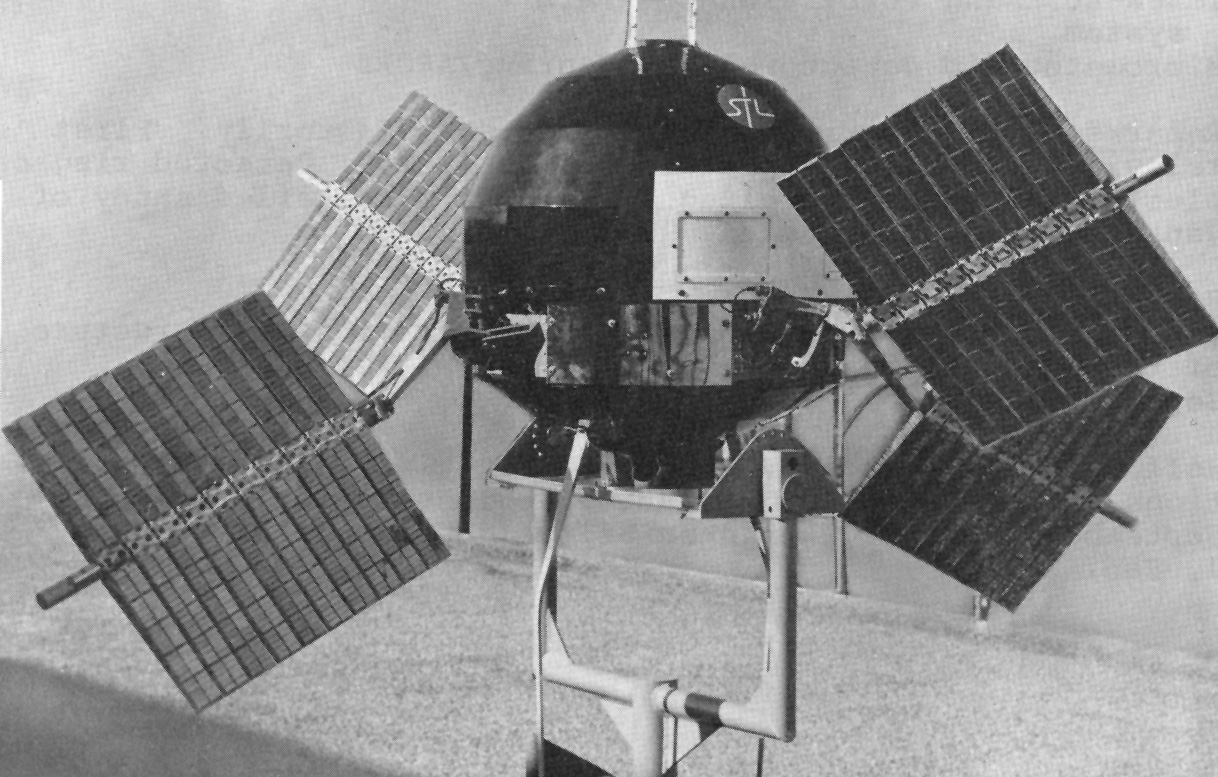
\includegraphics[scale = 1.65]{Figures/Explorer_6_paddles_up}
        \caption{NASA used solar cells on its spacecraft from the very beginning. For Example, Explorer 6, launched in 1959, had four arrays that folded out once in orbit. They provided power for months in space.}
        \label{fig:explorer}
    \end{figure}
    


\section{Aim}
    Our main objectives in this experiment are:
    \begin{enumerate}
        \item Study of I-V Characteristic of a solar cell illuminated by an incandescent lamp, at different frequencies,
        \item Study of I-V Characteristic of a solar cell illuminated by sun, at different frequencies,
        \item Study how the junction capacitance varies with applied reverse bias and to estimate the doping density as well as the built-in potential by analysing the C-V characteristic of a solar cell.
    \end{enumerate}
    
    
\section{Apparatus}
    The apparatus needed for this experiment is:
    \begin{enumerate}
        \item Solar cell/panel,
        \item Halogen lamp source as artificial light,
        \item Optical bench to position the solar panel and a clamp,
        \item Multimeters,
        \item Filter papers of various colors,
        \item Operational amplifier 0742 (TL072),
        \item Resistors and capacitors,
        \item Function generator and DC power supply
        \item Breadboard and
        \item Connecting wires
    \end{enumerate}


\section{Theory}
    Solar cell is the basic unit of solar energy generation system where electrical energy is
    extracted directly from light energy without any intermediate process. The working of a solar
    cell solely depends upon its photovoltaic effect, hence a solar cell also known as photovoltaic
    cell. A solar cell is basically a semiconductor p-n junction device. It is formed by joining p-
    type (high concentration of hole or deficiency of electron) and n-type (high concentration of
    electron) semiconductor material. at the junction excess electrons from n-type try to diffuse to
    p-side and vice-versa. Movement of electrons to the p-side exposes positive ion cores in n-
    side, while movement of holes to the n-side exposes negative ion cores in the p-side. This
    results in an electric field at the junction and forming the depletion region. When sunlight
    falls on the solar cell, photons with energy greater than band gap of the semiconductor are
    absorbed by the cell and generate electron-hole (e-h) pair. These e-h pairs migrate
    respectively to n- and p- side of the p0n junction due to electrostatic force of the field across
    the junction. In this way a potential difference is established between two sides of the cell.
    Typically a solar or photovoltaic cell has negative front contact and positive back contact. A
    semiconductor p-n junction is in the middle of these two contacts like a battery. If these two
    sides are connected by an external circuit, current will start flowing from positive to negative
    terminal of the solar cell. This is basic working principle of a solar cell. For silicon, the band
    gap at room temperature is $E_g = \SI{1.1}{\electronvolt}$ and the diffusion potential is $U_D = 0.5$ to $\SI{0.7}{\volt}$. Construction of a Si solar cell is depicted in figure (\ref{fig:cons}).
    \begin{figure}
        \centering
        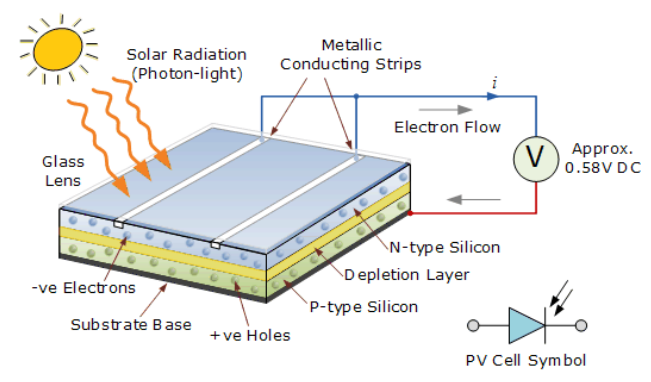
\includegraphics[scale = 0.62]{Figures/construction.png}
        \caption{Construction of a solar cell}
        \label{fig:cons}
    \end{figure}
    \begin{figure}
        \centering
        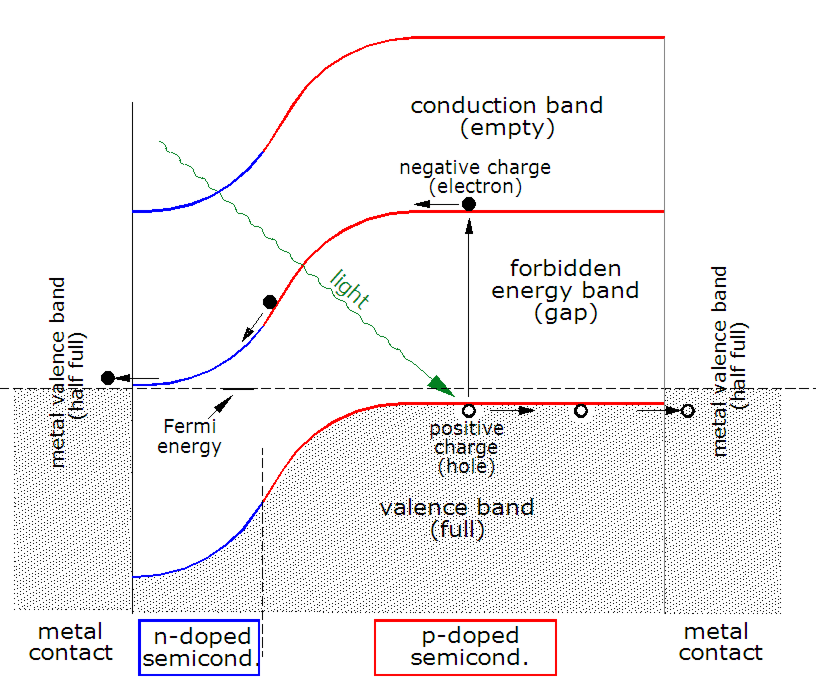
\includegraphics[scale = 0.3]{Figures/BandDiagramSolarCell-en.png}
        \caption{Band diagram of a silicon solar cell, corresponding to very low current (horizontal Fermi level), very low voltage (metal valence bands at same height), and therefore very low illumination}
        \label{fig:banddiagram}
    \end{figure}
    \subsection{Solar cell parameters}
        Materials scientists often characterise solar cells in terms of simple circuit analysis; these typically include a p-n junction diode, a shunt resistance and a series resistor. Therefore, electrical characterization using a combination of DC and AC techniques allows the scientist to measure each of these components within the cell. Furthermore, different cell chemistries are at various stages of development and therefore some systems still require a significant effort in understanding the underlying physics of the devices. For example, polycrystalline Silicon is well understood as it has benefited from over 40 years R\&D effort from the semiconductor industry. However, limitations due to cost and low theoretical efficiencies are driving scientists to seek new materials such as III-V compounds and polymeric systems in which the basic science is less mature. At present, scientists are engaged in a number of parallel strategies to improve the performance of next generation devices such as fundamental material characterization, multiple junction arrays and development of device structure. This necessitates the use of complex, accurate and flexible electrical characterization instruments that can meet the future demands of the scientists in this field.
        \par
        Photovoltaic solar cells convert the suns radiant light directly into electricity. With increasing demand for a clean energy source and the sun’s potential as a free energy source, has made solar energy conversion as part of a mixture of renewable energy sources increasingly important. As a result, the demand for efficient solar cells, which convert sunlight directly into electricity, is growing faster than ever before.
        \par
        Photovoltaic (PV) cells are made made almost entirely from semiconductor silicon that has been processed into an extremely pure crystalline material which absorbs the photons from sunlight.
        \par
        The photons hit the sillicon atoms releasing electrons causing an electric current to flow when the photoconductive cell is connected to an external load. For example, a battery. There are a variety of different measurements we can make to determine the solar cell’s performance, such as its power output and its conversion efficiency.
        \par
    \subsection{I-V characteristics of a solar cell}
    The Solar Cell I-V Characteristic Curves shows the current and voltage (I-V) characteristics of a particular photovoltaic (PV) cell, module or array. It gives a detailed description of its solar energy conversion ability and efficiency. Knowing the electrical I-V characteristics (more importantly $P_{max}$) of a solar cell, or panel is critical in determining the device’s output performance and solar efficiency.
    \par
    According to Lindholm \textit{et al.}, the I-V curve of a solar cell is the superposition of the I-V curve of the solar cell diode in the dark with the light-generated current. An understanding of the performance of a solar cell device can be gleaned with the I-V characterization technique. The voltage is ramped linearly or in staircase mode from the open circuit value ($V_{OC}$) to the Short Circuit Voltage ($V_{SC}$) and the generated current is measured. Depending upon the parameter of interest, the I-V characteristics are either performed under illumination at different light intensities or in the dark.
    \par
    This simple result contains a large amount of useful information and the following parameters can be extracted from this data including $I_{SC}$ or the short-circuit current, $J_{SC}$ or the short-circuit current density, $V_{OC}$ or the open circuit Voltage, $P_{max}$ or the maximum power point. $I_{max}$ or the current at $P_{max}$, $V_{max}$ or the voltage at $P_{max}$, $FF$ or the fill factor and $\eta$ or the conversion efficiency.
    \subsubsection{The Short-circuit current}
        The short-circuit current is the current through the solar cell when the voltage across the solar cell is zero (i.e., when the solar cell is short circuited). Usually written as ISC, the short-circuit current is shown in figure (\ref{fig:short}).
        \begin{figure}
            \centering
            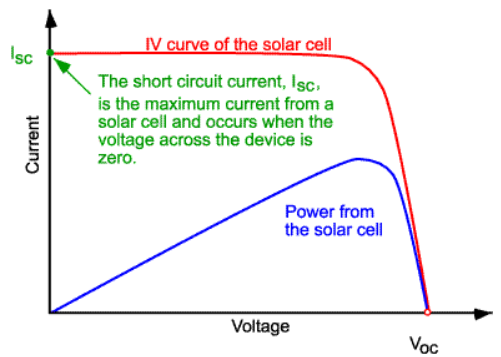
\includegraphics[scale = 0.65]{Figures/short-circuit.png}
            \caption{I-V curve of a solar cell showing the short-circuit current.}
            \label{fig:short}
        \end{figure}
        The short-circuit current is due to the generation and collection of light-generated carriers. For an ideal solar cell at most moderate resistive loss mechanisms, the short-circuit current and the light-generated current are identical. Therefore, the short-circuit current is the largest current which may be drawn from the solar cell.
        \par
        The short-circuit current depends on a number of factors like the area of the solar cell, the number of photons or the power of the incident light source, the spectrum of the incident light, the optical properties (absorption and reflection) of the solar cell and the minority-carrier collection probability of the solar cell, which depends chiefly on the surface passivation and the minority carrier lifetime in the base.
    \subsubsection{The Open-circuit Voltage}
        The open-circuit voltage, $V_{OC}$, is the maximum voltage available from a solar cell, and this occurs at zero current. The open-circuit voltage corresponds to the amount of forward bias on the solar cell due to the bias of the solar cell junction with the light-generated current. The open-circuit voltage is shown in figure (\ref{fig:open}).
        \begin{figure}
            \centering
            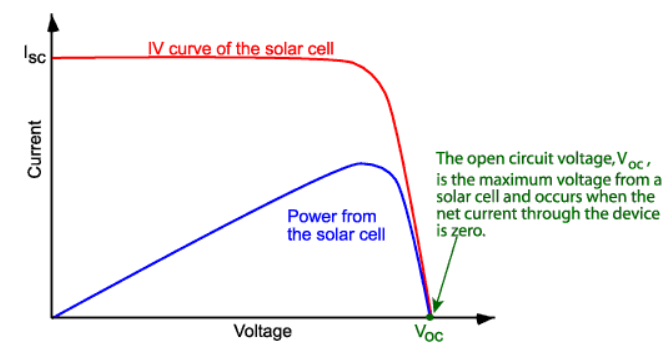
\includegraphics[scale = 0.61]{Figures/open-circuit.png}
            \caption{I-V curve of a solar cell showing the open-circuit voltage.}
            \label{fig:open}
        \end{figure}
    \subsubsection{Fill factor}
        The short-circuit current and the open-circuit voltage are the maximum current and voltage respectively from a solar cell. However, at both of these operating points, the power from the solar cell is zero. The "fill factor", more commonly known by its abbreviation "FF", is a parameter which, in conjunction with Voc and Isc, determines the maximum power from a solar cell. The FF is defined as the ratio of the maximum power from the solar cell to the product of Voc and Isc so that:
        \begin{equation}
            FF = \dfrac{P_{max}}{V_{OC} \times I_{SC}}
        \end{equation}
        Graphically, the FF is a measure of the "squareness" of the solar cell and is also the area of the largest rectangle which will fit in the IV curve.
    \subsubsection{The Shockley Diode Equation}
        The Shockley diode equation or the diode law, named after transistor co-inventor William Shockley of Bell Telephone Laboratories, gives the I–V (current-voltage) characteristic of an idealized diode in either forward or reverse bias (applied voltage). Illuminating the cell adds to the normal dark currents in the diode so that the diode law becomes:
        \begin{equation}
            I = I_0 \Big[ \exp \big( \dfrac{qv}{nkT}\big) -1 \Big] - I_L
        \end{equation}
        where $I_0$ is the dark saturation current or the diode leakage current in absence of light, $q$ is the electric charge, $V$ is the applied voltage across the diode terminals, $n$ is the ideality factor, $k$ is the Boltzmann's constant, $T$ is the temperature and $I_L$ is the light generated current.
    \subsubsection{Experimental set-up}
        A typical circuit for measuring I-V characteristics is shown in figure (\ref{fig:iv-cir}).
        \begin{figure}
            \centering
            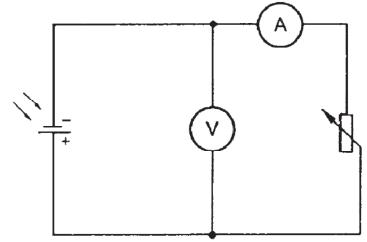
\includegraphics{Figures/ivcircuit.png}
            \caption{Caption}
            \label{fig:iv-cir}
        \end{figure}
        \begin{figure}
            \centering
            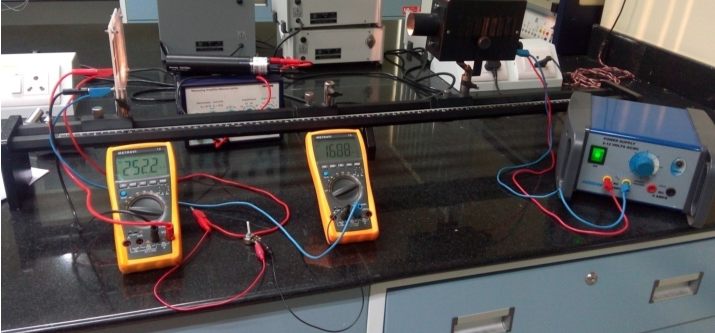
\includegraphics[scale = 0.55]{Figures/ivarr.png}
            \caption{Experimental set-up for I-V characterization of solar cell illuminated by lamp.}
            \label{fig:ivarr}
        \end{figure}
    \subsubsection{Efficiency}
        The efficiency is the most commonly used parameter to compare the performance of one solar cell to another. Efficiency is defined as the ratio of energy output from the solar cell to input energy from the sun. In addition to reflecting the performance of the solar cell itself, the efficiency depends on the spectrum and intensity of the incident sunlight and the temperature of the solar cell.
        \begin{figure}
            \centering
            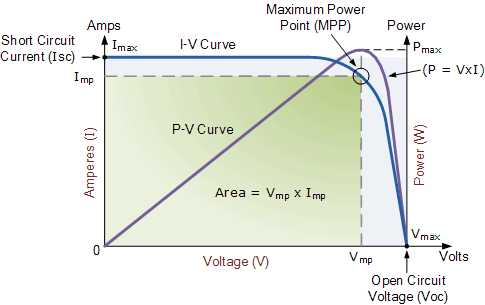
\includegraphics[scale = 0.5]{Figures/alt120.png}
            \caption{A typical I-V curve and power curve for a solar cell.}
            \label{fig:typicaliv}
        \end{figure}
    
    \subsection{C-V characteristics of a solar cell}
        Capacitance voltage measurements can be used to characterise fundamental properties of solar cells including an estimate of the charge carrier density and the drive level capacitance profile.
        \par
        When a p-n junction is reverse biased, uncompensated acceptor ions in the p- side of the junction and an equal number of ionized donors on the n- side of junction form the space charge region. Since there are no mobile carriers in this region, only the free carriers at the edge of the depletion region can respond to the externally applied ac field. The junction thus resembles a parallel plate capacitor, whose capacitance is specified as
        \begin{equation}
        \label{eq:Cap}
            C = \Bigg| \dfrac{dQ}{dV_{DC}} \Bigg| = \dfrac{\epsilon_0 \epsilon_s A}{x_d}
        \end{equation}
        where $Q$ is the charge (free charge carriers) on either side of the junction, $V_{DC}$ is the applied voltage, $\epsilon_s$ is the dielectric constant of the semiconductor, $\epsilon_0$ is the permittivity of free space, and $A$ is the area of the p-n junction. The depletion region width, $x_d$, for a reverse biased junction with constant doping density $N_d$ is given by
        \begin{equation}
        \label{eq:xd}
            x_d = \sqrt{\dfrac{2 \epsilon_0 \epsilon_s (V_{bi} + V_{DC})}{q N_d}}
        \end{equation}
        $V_{bi}$ is the built-in voltage, $q$ is the charge on an electron ($\SI{1.6e-19}{\coulomb}$) and $N_d$ is the doping density. From equations (\ref{eq:Cap}) and (\ref{eq:xd}), it follows that
        \begin{equation}
            \dfrac{1}{C^2} = \Big( \dfrac{x_d}{\epsilon_0 \epsilon_s A} \Big)^2 = \dfrac{2 (V_{bi} + V_{DC})}{q \epsilon_0 \epsilon_s A^2 N_d}
        \end{equation}
        A plot of $1/C^2$ versus $V_{DC}$ is a straight line with slope $d(1/C^2)/dV = 2/(q \epsilon_0 \epsilon_s A^2 N_d)$. By obtaining this plot, one can easily find doping density $N_d$ from the slope. The built-in potential $V_{bi}$ could be estimated from either the $Y$-axis intercept ($2 V_{bi}/(q \epsilon_0 \epsilon_s A^2 N_d)$).
        \subsubsection{Mechanism}
            The circuit diagram for C-V characterizations of the solar cell is given in figure (\ref{fig:cv-cir}). 
            \begin{figure}
                \centering
                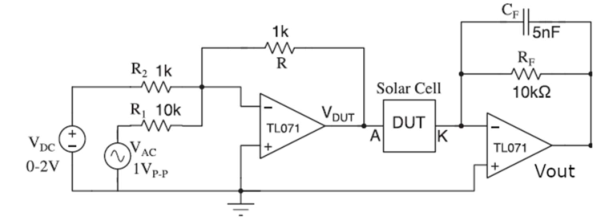
\includegraphics[scale = 0.6]{Figures/cvcircuit.png}
                \caption{Circuit to measure CV data}
                \label{fig:cv-cir}
            \end{figure}
            \par
            The capacitance of the solar cell (Device under test, DUT) depends strongly on the applied DC voltage. Since the experiment involves measurement of the C-V profile of the capacitor, the circuit must also be designed to apply an additional DC voltage across the capacitor (solar cell) that can be varied, while measuring the AC current to extract the capacitance. In our setup, we apply a variable DC bias and a small AC signal (small enough not to perturb DC bias and not affect the charge polarization due to the DC bias) to the DUT (Device Under Test). This is accomplished by using a basic inverting summing amplifier that adds the variable DC voltage (with unity gain $R/R_2$) and the small signal AC voltage (with attenuation factor $1/10 = R/R_1$), the output voltage of which is then connected to the DUT. The voltage $V_{DUT}$ in figure (\ref{fig:cv-cir}) is thus given by the following equation
            \begin{equation}
                V_{DUT} = - R \Bigg( \dfrac{V_{DC}}{R_2} + \dfrac{V_{AC}}{R_1} \Bigg)
            \end{equation}
            \par
            The AC voltage amplitude across the DUT (solar cell) is thus one tenth of the applied input DC voltage (smaller AC voltage can also be applied but we are limited by the sensitivity of our measuring instrument). One end (Anode, A) of the solar cell is connected to the output of the summing circuit while the other end (cathode, K) is virtually grounded due to negative feedback in the op-amp circuit. Current through a capacitor is proportional to the applied AC sinusoidal voltage. We use a transimpedance amplifier (I to V converter) so that the current flowing through the capacitor is converted into voltage, a multimeter. The transimpedance amplifier generates a voltage output that is proportional to the DUT capacitance ($C_{DUT}$) and $V_{DUT}$. The magnitude of this voltage is given by following equation
            \begin{equation}
                V_{OUT} = V_{DUT} \dfrac{C_{DUT}}{C_F} \dfrac{1}{\sqrt{1 + \dfrac{1}{(\omega R_F C_F)^2}}}
            \end{equation}
    \subsection{Integrators and Differentiators}
        The electronic circuits which perform the mathematical operations such as differentiation and integration are called as differentiator and integrator, respectively. A differentiator is an electronic circuit that produces an output equal to the first derivative of its input.
        \par
        An op-amp based differentiator produces an output, which is equal to the differential of input voltage that is applied to its inverting terminal. The circuit diagram of an op-amp based differentiator is shown in figure (\ref{fig:diff}).
        \begin{figure}
            \centering
            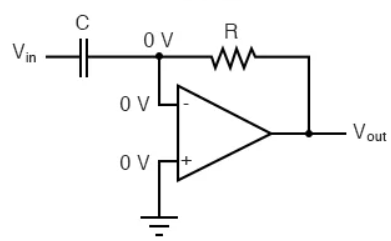
\includegraphics{Figures/differentiator.png}
            \caption{Circuit diagram of a differentiator circuit}
            \label{fig:diff}
        \end{figure}
        In the above circuit, the non-inverting input terminal of the op-amp is connected to ground. That means zero volts is applied to its non-inverting input terminal.
        \par
        According to the virtual short concept, the voltage at the inverting input terminal of opamp will be equal to the voltage present at its non-inverting input terminal. So, the voltage at the inverting input terminal of op-amp will be zero volts. 
        \par
        The nodal equation at the inverting input terminal's node is
        \begin{equation}
            \begin{split}
                C \dfrac{d (0-V_i)}{dt} &+ \dfrac{0-V_0}{R} = 0 \\
                \implies - C \dfrac{dV_i}{dt} &= \dfrac{V_0}{R} \\
                \implies V_0 &= -RC \dfrac{dV_i}{dt}
            \end{split}
        \end{equation}
        Thus, the op-amp based differentiator circuit shown above will produce an output, which is the differential of input voltage $V_i$, when the magnitudes of impedances of resistor and capacitor are reciprocal to each other.
        \par
        An integrator is an electronic circuit that produces an output that is the integration of the applied input. An op-amp based integrator produces an output, which is an integral of the input voltage applied to its inverting terminal. The circuit diagram of an op-amp based integrator is shown in figure (\ref{fig:int}).
        \begin{figure}
            \centering
            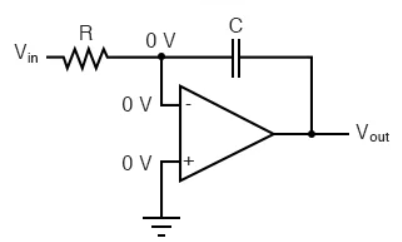
\includegraphics{Figures/integrator.png}
            \caption{Circuit diagram of a differentiator circuit}
            \label{fig:int}
        \end{figure}
        In the circuit shown above, the non-inverting input terminal of the op-amp is connected to ground. That means zero volts is applied to its non-inverting input terminal.
        \par
        According to virtual short concept, the voltage at the inverting input terminal of op-amp will be equal to the voltage present at its non-inverting input terminal. So, the voltage at the inverting input terminal of op-amp will be zero volts. The nodal equation at the inverting input terminal is
        \begin{equation}
            \begin{split}
                \dfrac{0-V_i}{R} &+ C \dfrac{d(0-V_0)}{dt} = 0 \\
                \implies -\dfrac{V_i}{R} &= C \dfrac{V_0}{dt} \\
                \implies \int dv_0 &= \int \Bigg( -\dfrac{V_i}{RC} \Bigg) \\
                \implies V_0 &= - \dfrac{1}{RC} \int V_t dt
            \end{split}
        \end{equation}
        So, the op-amp based integrator circuit discussed above will produce an output, which is the integral of input voltage $V_i$, when the magnitude of impedances of resistor and capacitor are reciprocal to each other.
\section{Observations}
    The following preliminary observations were made
    \begin{enumerate}
        \item For the I-V characterization, the supply voltage to the incandescent halogen lamp was $\SI{6}{\volt}$.
        \item The distance between lamp and solar cell was kept around $\SI{5}{\centi \metre}$.
        \item The frequency of the function generator for C-V characterization was set to be at $\SI{2}{\kilo \hertz}$.
        \item The circuit components (resistors, capacitors) of C-V characterization are marked in the figure (\ref{fig:cv-cir}).
        \item  Electronic charge on the electron is $q = \SI{1.6e-19}{\coulomb}$ and permittivity of free space is $\epsilon_0 = \SI{8.85e-12}{\per \metre \cubed \per \kilogram \second\tothe{4} \ampere \squared}$.
        \item The dielectric constant for Si (solar cell) is $\epsilon_s = 11.7$.
        \item The area of the p-n junction is $A = \SI{61.75}{\centi \metre \squared}$.
    \end{enumerate}
    The data for I-V characterization of the solar cell illuminated by the incandescent halogen lamp is tabulated in table (\ref{tab:iv-lamp}). The data for I-V characterization of the solar cell illuminated by the sun is tabulated in table (\ref{tab:iv-sun}). The I-V curves for illumination by the incandescent halogen lamp against various filters are plotted in figure (\ref{fig:iv-lamp}) and for illumination by the sun in figure (\ref{fig:iv-sun}). The parameters so obtained from the I-V characteristic curves are tabulated in tables (\ref{tab:iv-1}) and (\ref{tab:iv-2}).
    \par
    The data for C-V characterization of the solar cell in light conditions is tabulated in table (\ref{tab:cv-light}) and in dark conditions in table (\ref{tab:cv-dark}). The corresponding plots of $C$ versus $V_{DC}$ and $1/C^2$ versus $V_{DC}$ are plotted in figures (\ref{fig:cv-light}) and (\ref{fig:cv-dark}).
    \begin{table*}[]
    \caption{I-V characterization of the solar cell illuminated by an incandescent halogen lamp with various filters}
    \label{tab:iv-lamp}
    \setlength{\tabcolsep}{8pt}
    \begin{tabular}{@{}cccccccccccccc@{}}
    \toprule
    \multicolumn{2}{c}{\textbf{No Filter}} &  & \multicolumn{2}{c}{\textbf{Red filter}} &  & \multicolumn{2}{c}{\textbf{Green filter}} &  & \multicolumn{2}{c}{\textbf{Yellow filter}} &  & \multicolumn{2}{c}{\textbf{Pink filter}} \\ \cmidrule(r){1-2} \cmidrule(lr){4-5} \cmidrule(lr){7-8} \cmidrule(lr){10-11} \cmidrule(l){13-14} 
    \begin{tabular}[c]{@{}c@{}}\textit{Voltage}\\ ($\si{\volt}$)\end{tabular} & \begin{tabular}[c]{@{}c@{}}\textit{Current} \\ ($\si{\milli \ampere}$)\end{tabular} &  & \begin{tabular}[c]{@{}c@{}}\textit{Voltage}\\ ($\si{\volt}$)\end{tabular} & \begin{tabular}[c]{@{}c@{}}\textit{Current} \\ ($\si{\milli \ampere}$)\end{tabular} &  & \begin{tabular}[c]{@{}c@{}}\textit{Voltage}\\ ($\si{\volt}$)\end{tabular} & \begin{tabular}[c]{@{}c@{}}\textit{Current} \\ ($\si{\milli \ampere}$)\end{tabular} &  & \begin{tabular}[c]{@{}c@{}}\textit{Voltage}\\ ($\si{\volt}$)\end{tabular} & \begin{tabular}[c]{@{}c@{}}\textit{Current} \\ ($\si{\milli \ampere}$)\end{tabular} &  & \begin{tabular}[c]{@{}c@{}}\textit{Voltage}\\ ($\si{\volt}$)\end{tabular} & \begin{tabular}[c]{@{}c@{}}\textit{Current} \\ ($\si{\milli \ampere}$)\end{tabular} \\ \midrule
    3.759 & 0.037 &  & 3.73 & 0.037 &  & 3.7 & 0.067 &  & 3.77 & 0.038 &  & 3.93 & 0.039 \\
    3.742 & 0.044 &  & 3.7 & 0.052 &  & 3.68 & 0.076 &  & \multirow{2}{*}{3.73} & \multirow{2}{*}{0.058} &  & 3.84 & 0.058 \\
    3.726 & 0.051 &  & 3.68 & 0.064 &  & 3.65 & 0.09 &  &  &  &  & 3.81 & 0.074 \\
    3.69 & 0.065 &  & \multirow{2}{*}{3.64} & \multirow{2}{*}{0.079} &  & 3.563 & 0.118 &  & \multirow{2}{*}{3.7} & \multirow{2}{*}{0.075} &  & 3.77 & 0.094 \\
    3.643 & 0.083 &  &  &  &  & 3.545 & 0.127 &  &  &  &  & 3.74 & 0.112 \\
    3.6 & 0.095 &  & \multirow{2}{*}{3.578} & \multirow{2}{*}{0.1} &  & \multirow{2}{*}{3.476} & \multirow{2}{*}{0.148} &  & \multirow{2}{*}{3.635} & \multirow{2}{*}{0.1} &  & 3.69 & 0.134 \\
    3.552 & 0.103 &  &  &  &  &  &  &  &  &  &  & 3.643 & 0.154 \\
    3.492 & 0.12 &  & \multirow{2}{*}{3.501} & \multirow{2}{*}{0.125} &  & \multirow{2}{*}{3.395} & \multirow{2}{*}{0.168} &  & \multirow{2}{*}{3.589} & \multirow{2}{*}{0.118} &  & 3.572 & 0.179 \\
    3.434 & 0.133 &  &  &  &  &  &  &  &  &  &  & 3.478 & 0.205 \\
    \multirow{2}{*}{3.251} & \multirow{2}{*}{0.167} &  & \multirow{2}{*}{3.424} & \multirow{2}{*}{0.145} &  & \multirow{2}{*}{3.311} & \multirow{2}{*}{0.185} &  & \multirow{2}{*}{3.523} & \multirow{2}{*}{0.138} &  & 3.371 & 0.226 \\
     &  &  &  &  &  &  &  &  &  &  &  & 3.176 & 0.249 \\
    \multirow{2}{*}{2.944} & \multirow{2}{*}{0.203} &  & \multirow{2}{*}{3.268} & \multirow{2}{*}{0.177} &  & \multirow{2}{*}{3.182} & \multirow{2}{*}{0.203} &  & \multirow{2}{*}{3.386} & \multirow{2}{*}{0.17} &  & 2.739 & 0.267 \\
     &  &  &  &  &  &  &  &  &  &  &  & 2.262 & 0.277 \\
    2.543 & 0.219 &  & \multirow{2}{*}{3.123} & \multirow{2}{*}{0.196} &  & \multirow{2}{*}{3.017} & \multirow{2}{*}{0.214} &  & \multirow{2}{*}{3.248} & \multirow{2}{*}{0.192} &  & 1.636 & 0.289 \\
    1.745 & 0.231 &  &  &  &  &  &  &  &  &  &  & 1.365 & 0.297 \\
    1.426 & 0.235 &  & \multirow{2}{*}{2.555} & \multirow{2}{*}{0.221} &  & \multirow{2}{*}{2.348} & \multirow{2}{*}{0.233} &  & \multirow{2}{*}{2.833} & \multirow{2}{*}{0.218} &  & 1.257 & 0.303 \\
    0.748 & 0.247 &  &  &  &  &  &  &  &  &  &  & 1.07 & 0.309 \\
    0.669 & 0.249 &  & \multirow{2}{*}{0.906} & \multirow{2}{*}{0.254} &  & 1.78 & 0.243 &  & \multirow{2}{*}{0.888} & \multirow{2}{*}{0.246} &  & 0.723 & 0.32 \\
    0.474 & 0.255 &  &  &  &  & 1.078 & 0.257 &  &  &  &  & 0.284 & 0.337 \\
    0.328 & 0.259 &  & \multirow{2}{*}{0.245} & \multirow{2}{*}{0.262} &  & 0.65 & 0.268 &  & \multirow{2}{*}{0.085} & \multirow{2}{*}{0.257} &  & 0.265 & 0.343 \\
    0.272 & 0.26 &  &  &  &  & 0.273 & 0.279 &  &  &  &  & 0.133 & 0.35 \\
    0.1 & 0.266 &  & 0.076 & 0.266 &  & 0.098 & 0.282 &  & 0.068 & 0.26 &  & 0.089 & 0.353 \\
    0.061 & 0.268 &  & 0.059 & 0.268 &  & 0.059 & 0.285 &  & 0.054 & 0.263 &  & 0.064 & 0.356 \\ \bottomrule
    \end{tabular}
    \end{table*}
    
    \begin{figure*}
        \centering
        \begin{subfigure}[b]{0.49\textwidth}
            \centering
            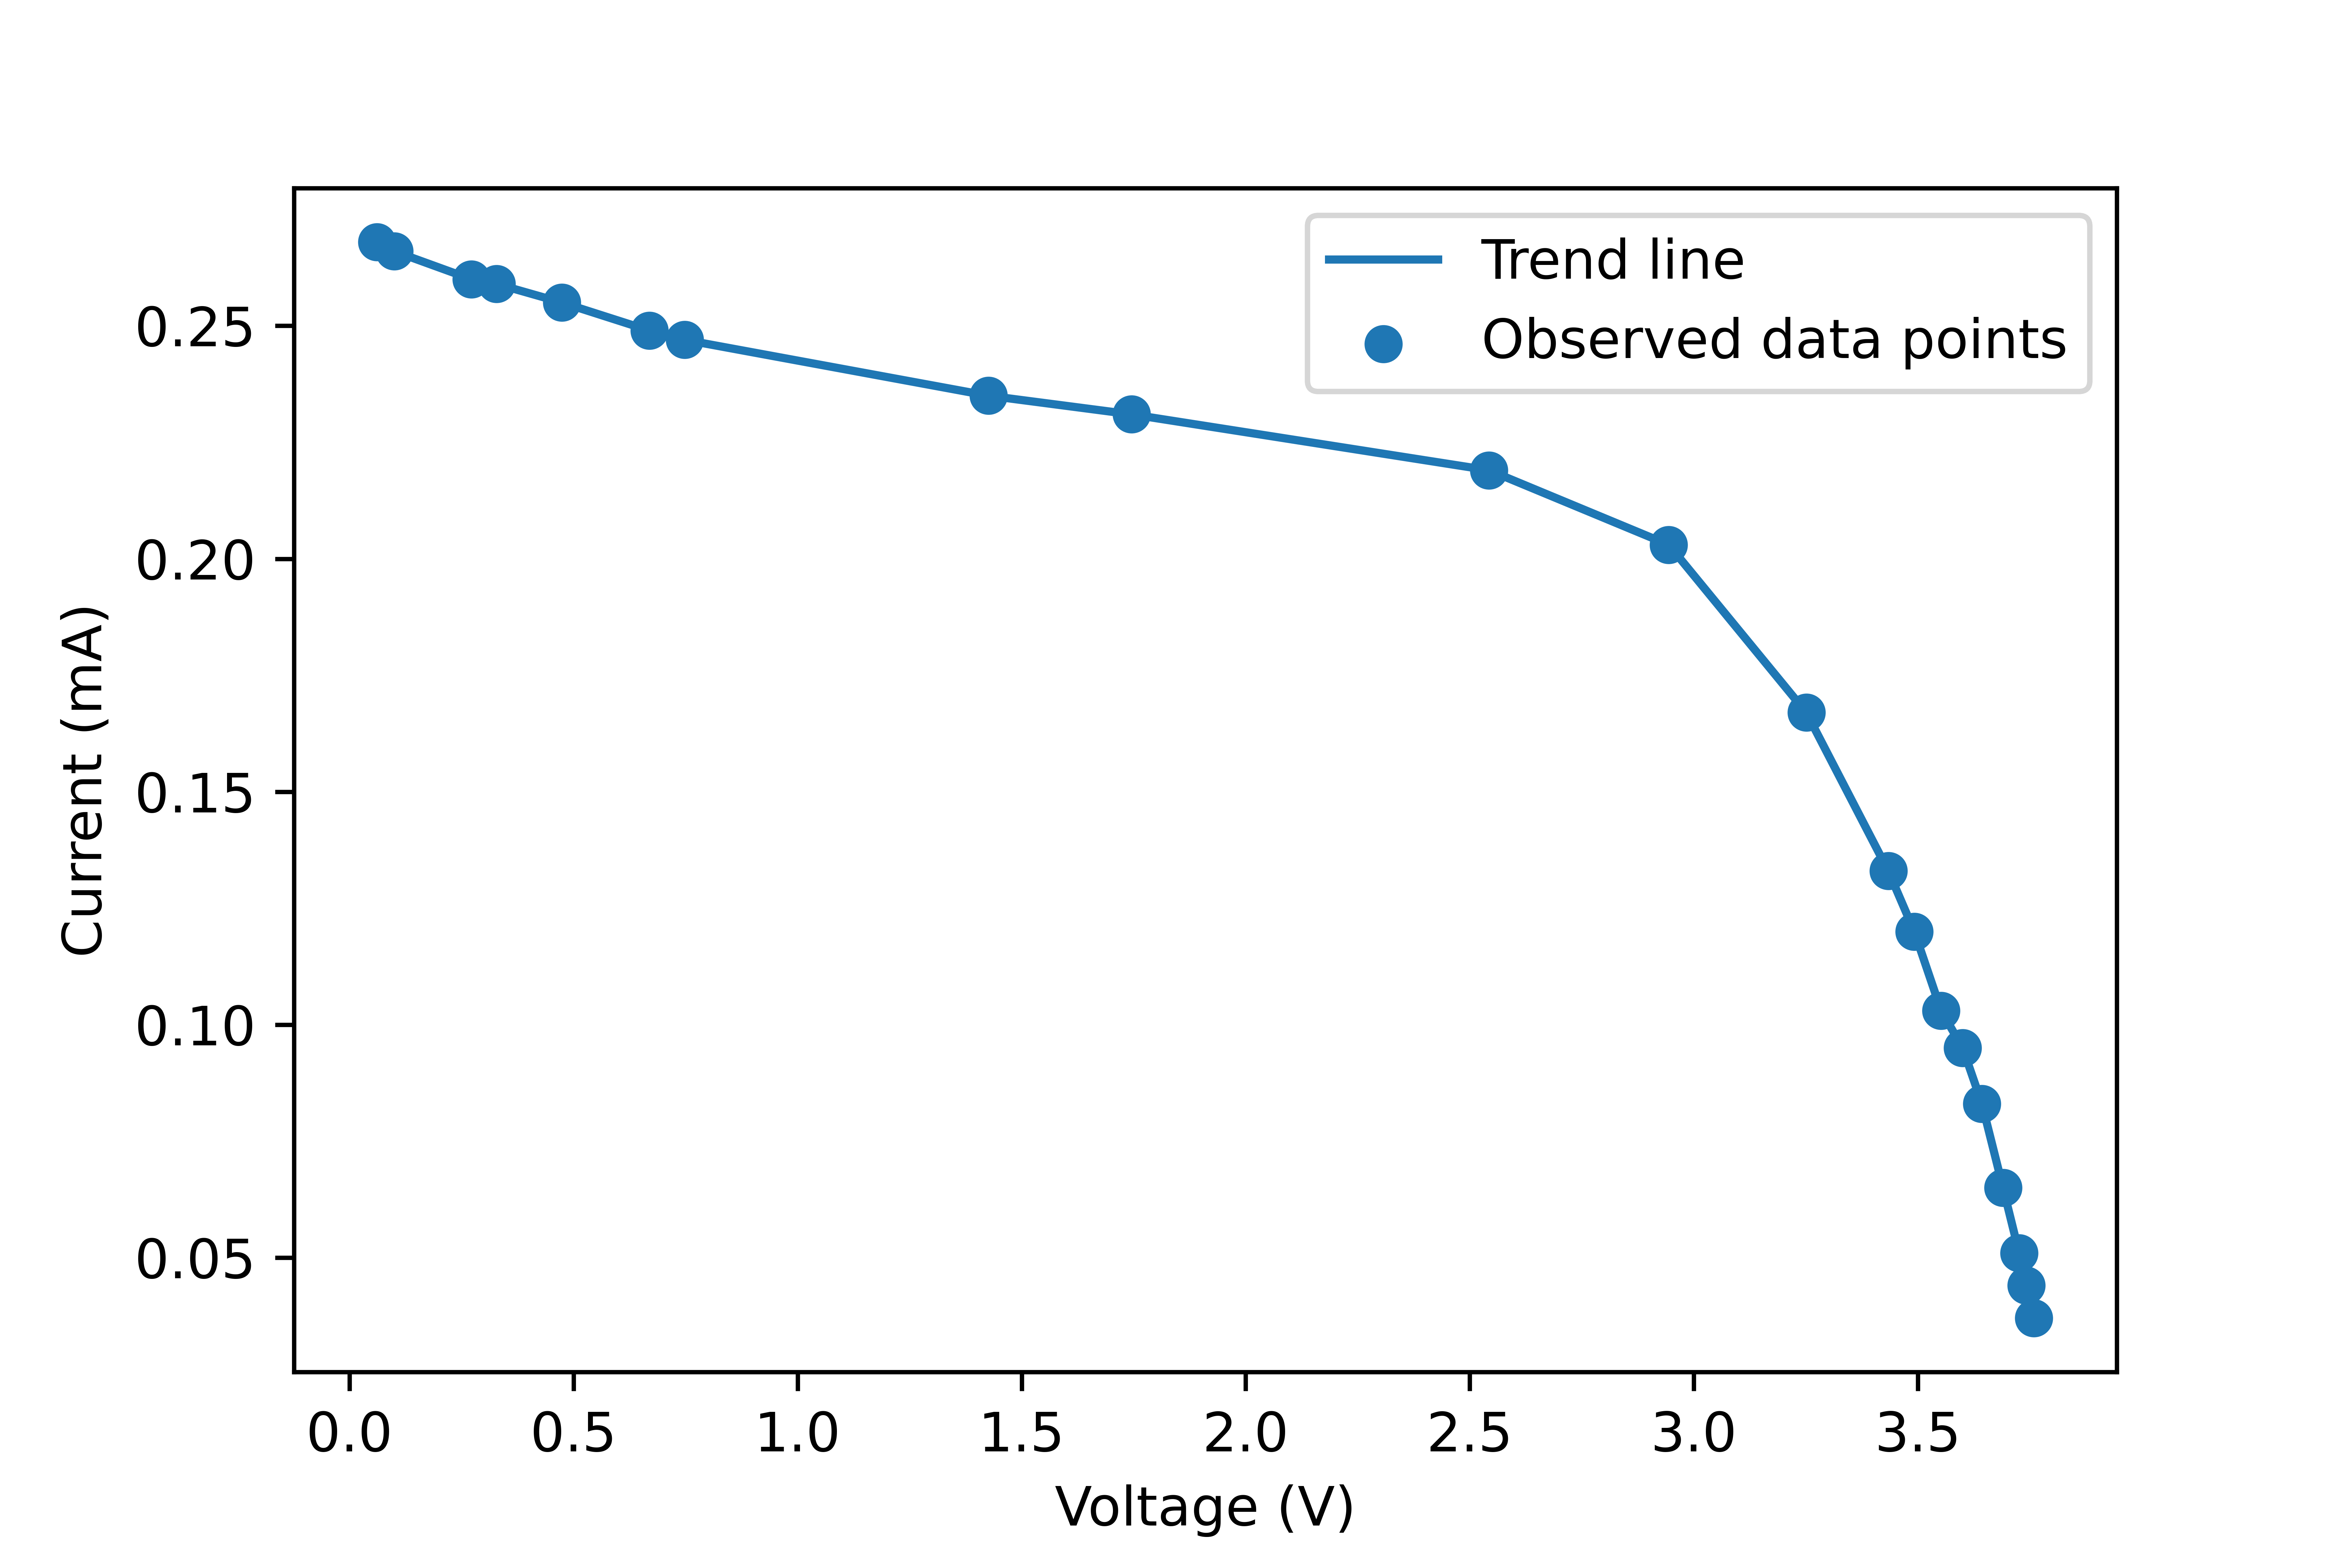
\includegraphics[scale = 0.54]{Figures/plot-iv-lamp-nofilter.png}
            \caption{With no filter}
            \label{fig:iv-lamp-nofilter}
        \end{subfigure}
        \hfill
        \begin{subfigure}[b]{0.49\textwidth}
            \centering
            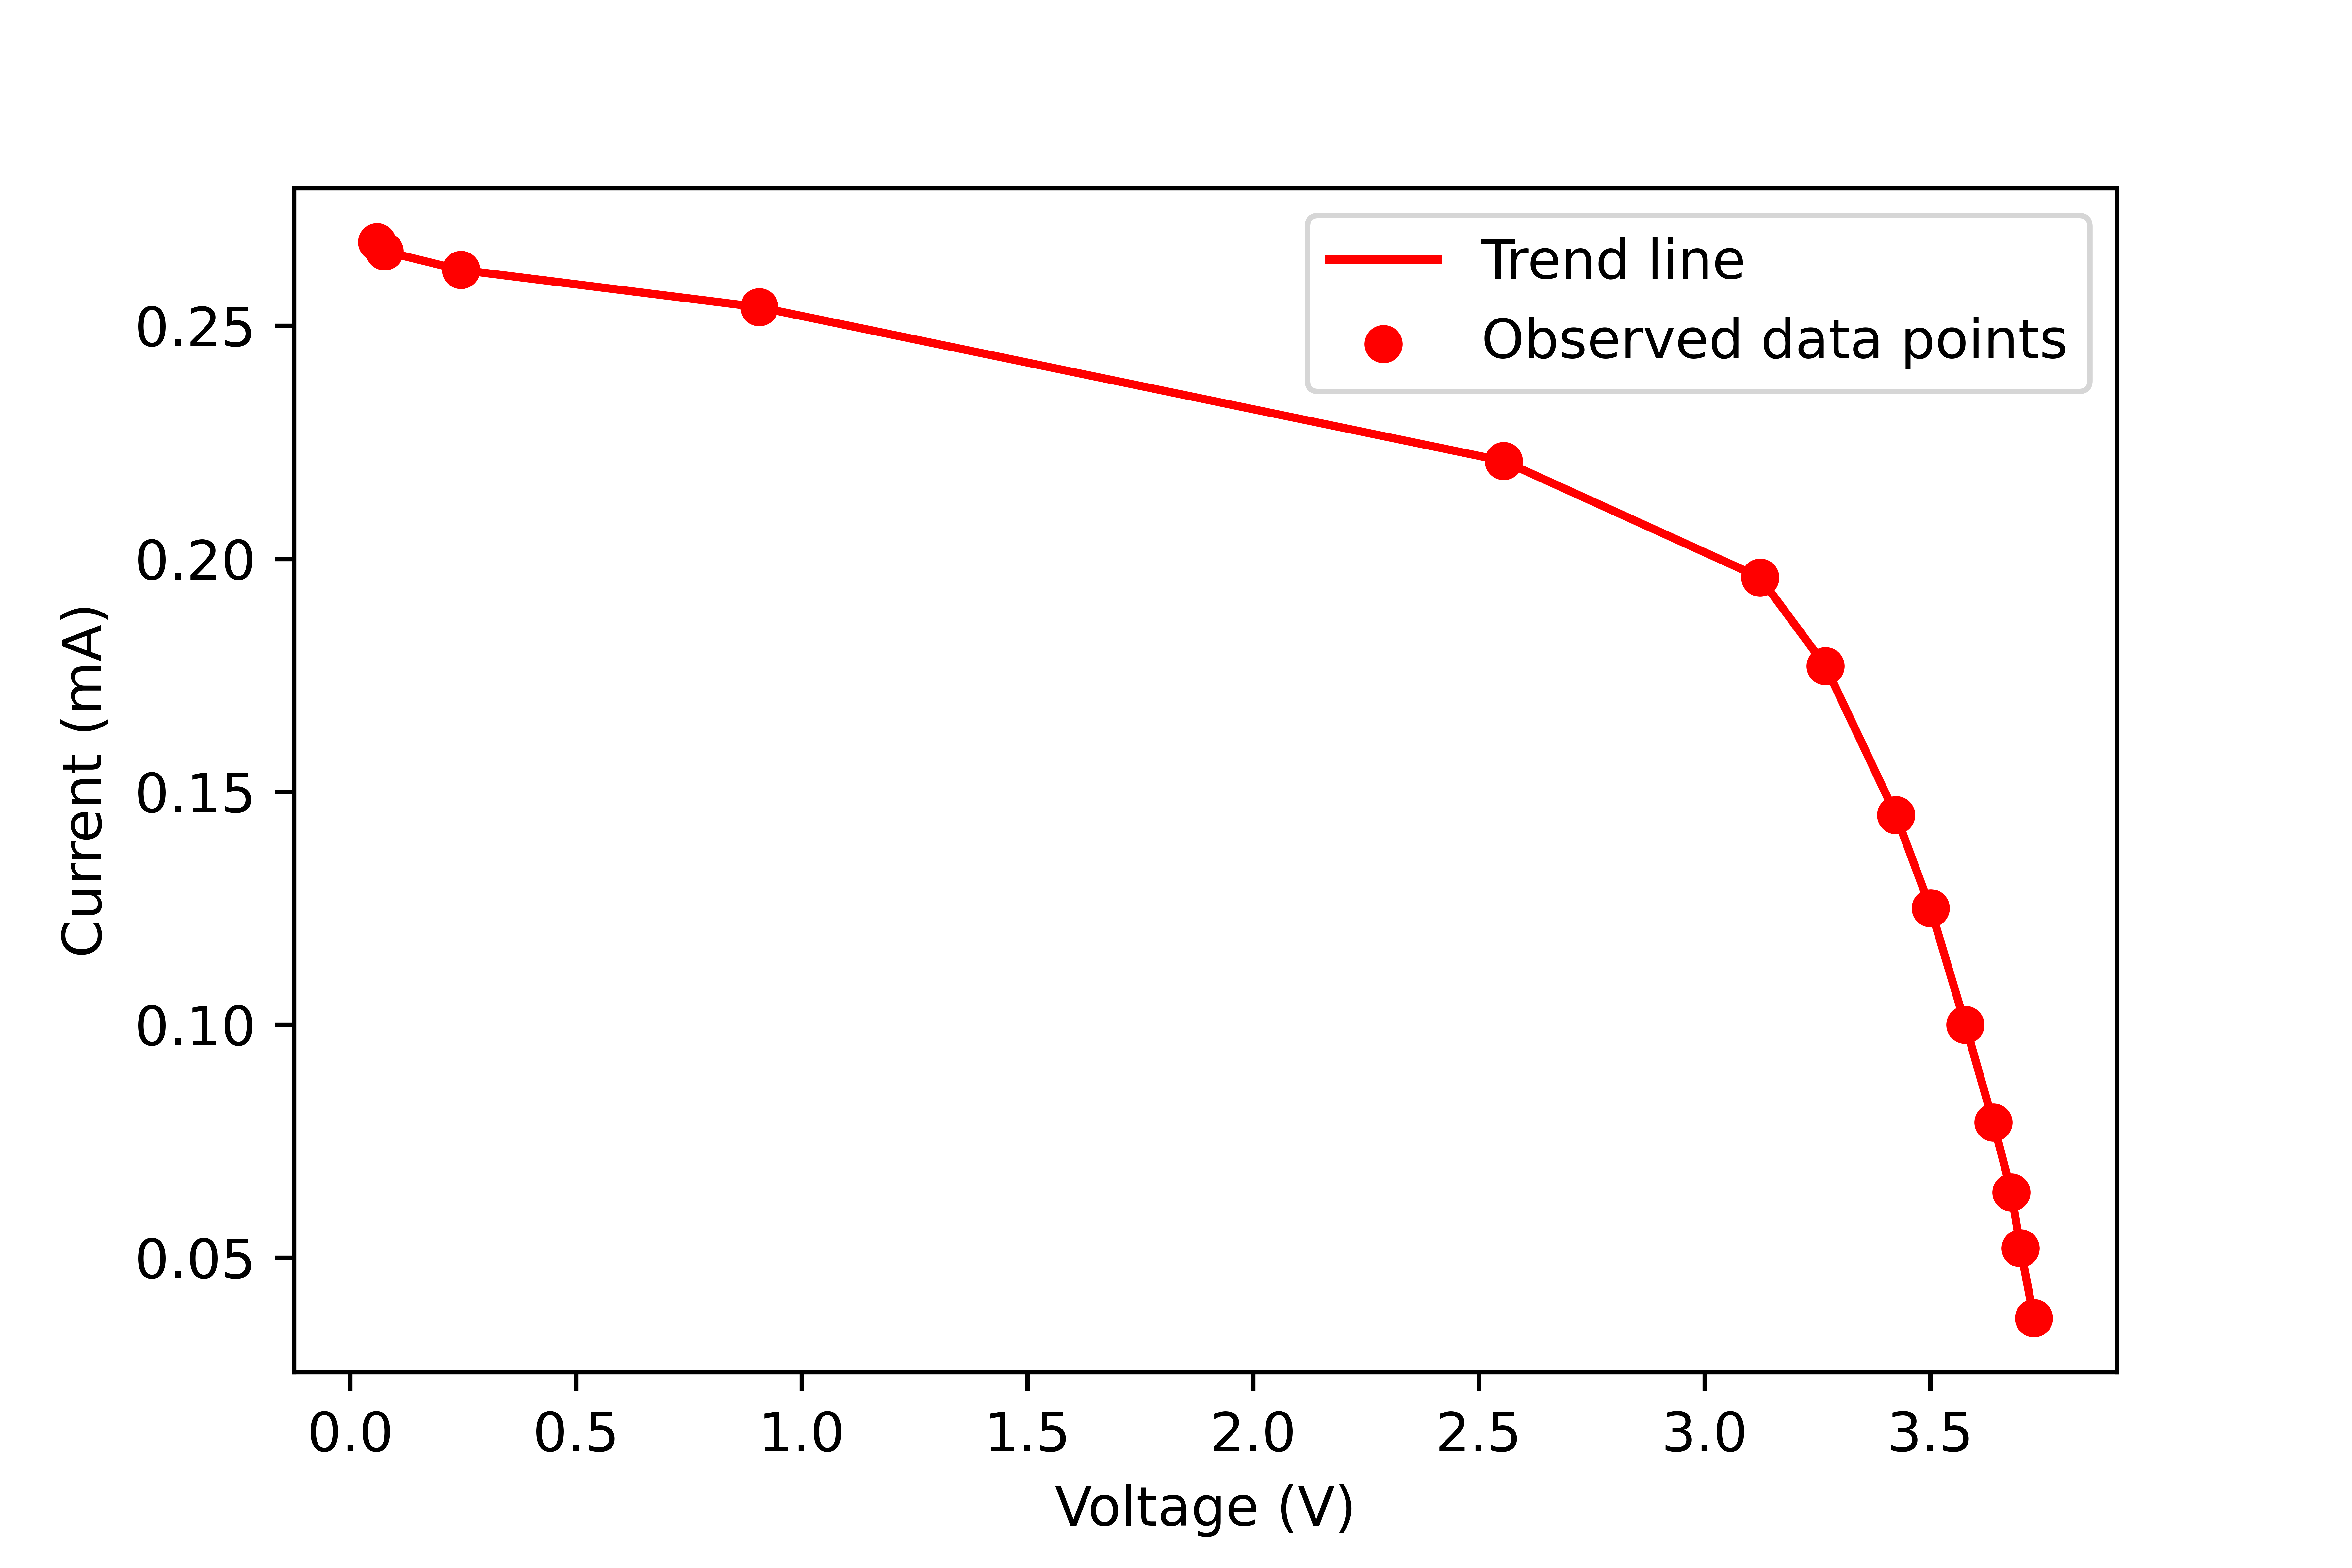
\includegraphics[scale = 0.54]{Figures/plot-iv-lamp-red.png}
            \caption{With red filter}
            \label{fig:iv-lamp-red}
        \end{subfigure}
        \hfill
        \begin{subfigure}[b]{0.49\textwidth}
            \centering
            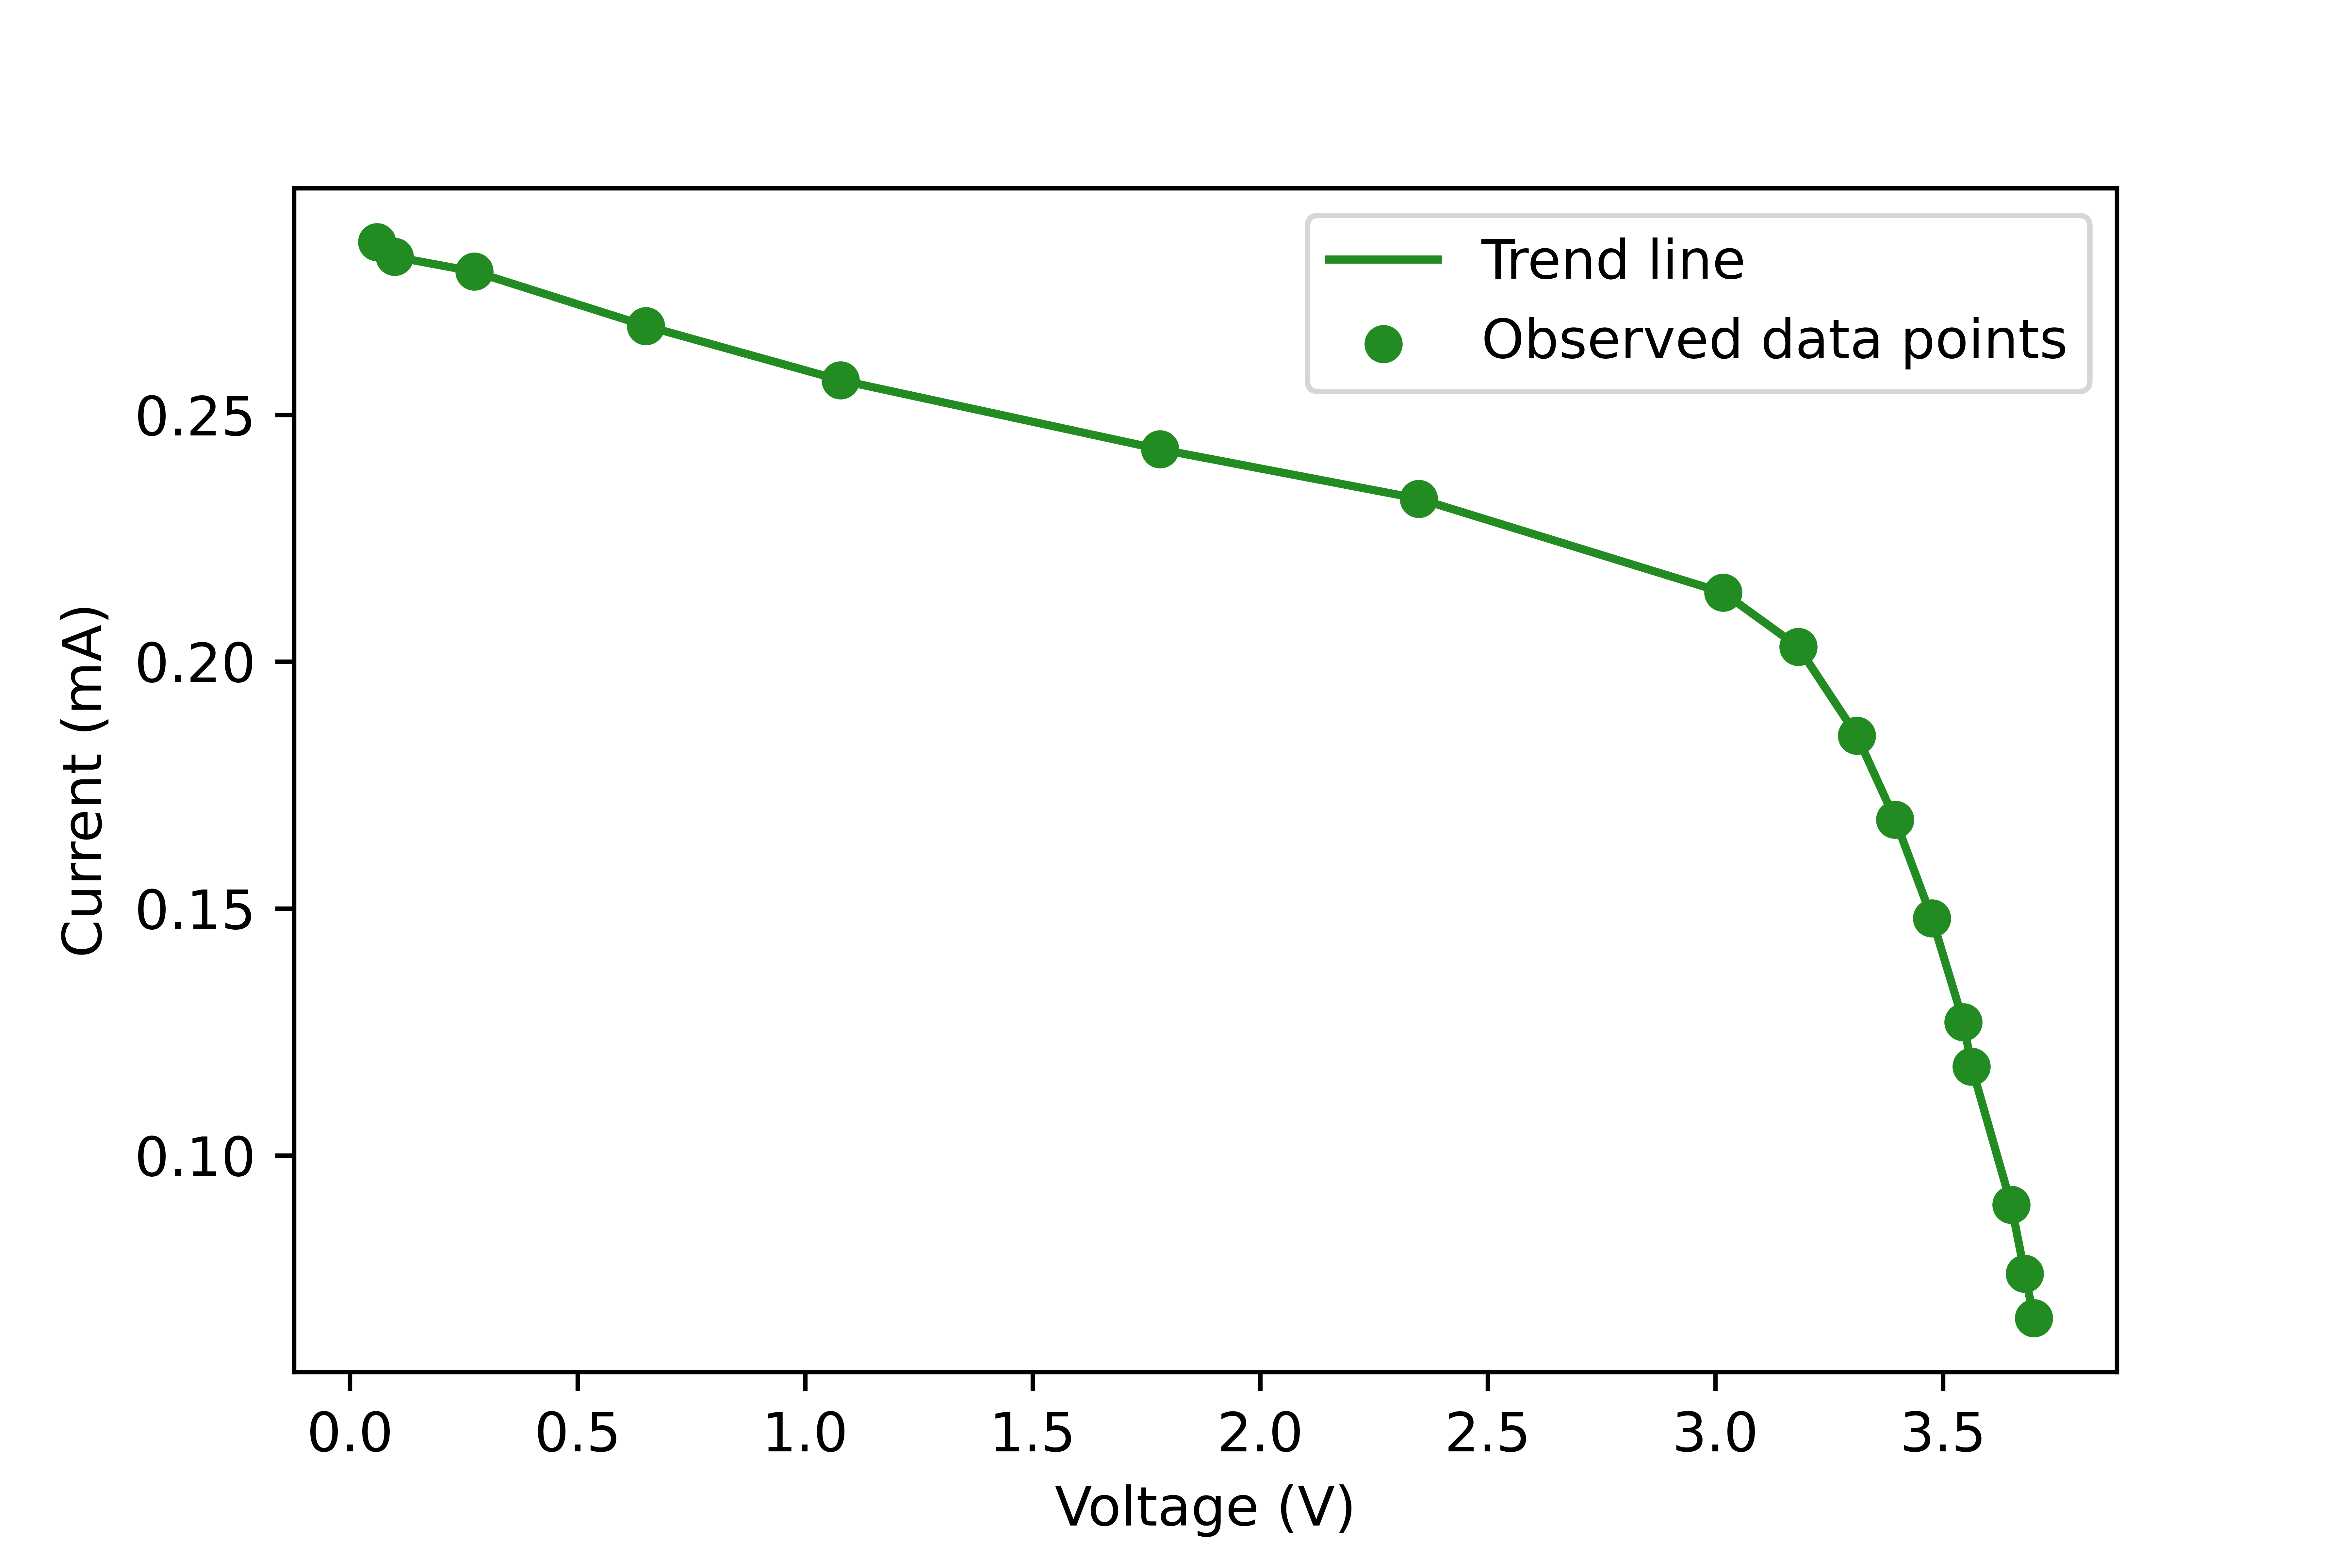
\includegraphics[scale = 0.54]{Figures/plot-iv-lamp-green.png}
            \caption{With green filter}
            \label{fig:iv-lamp-green}
        \end{subfigure}
        \hfill
        \begin{subfigure}[b]{0.49\textwidth}
            \centering
            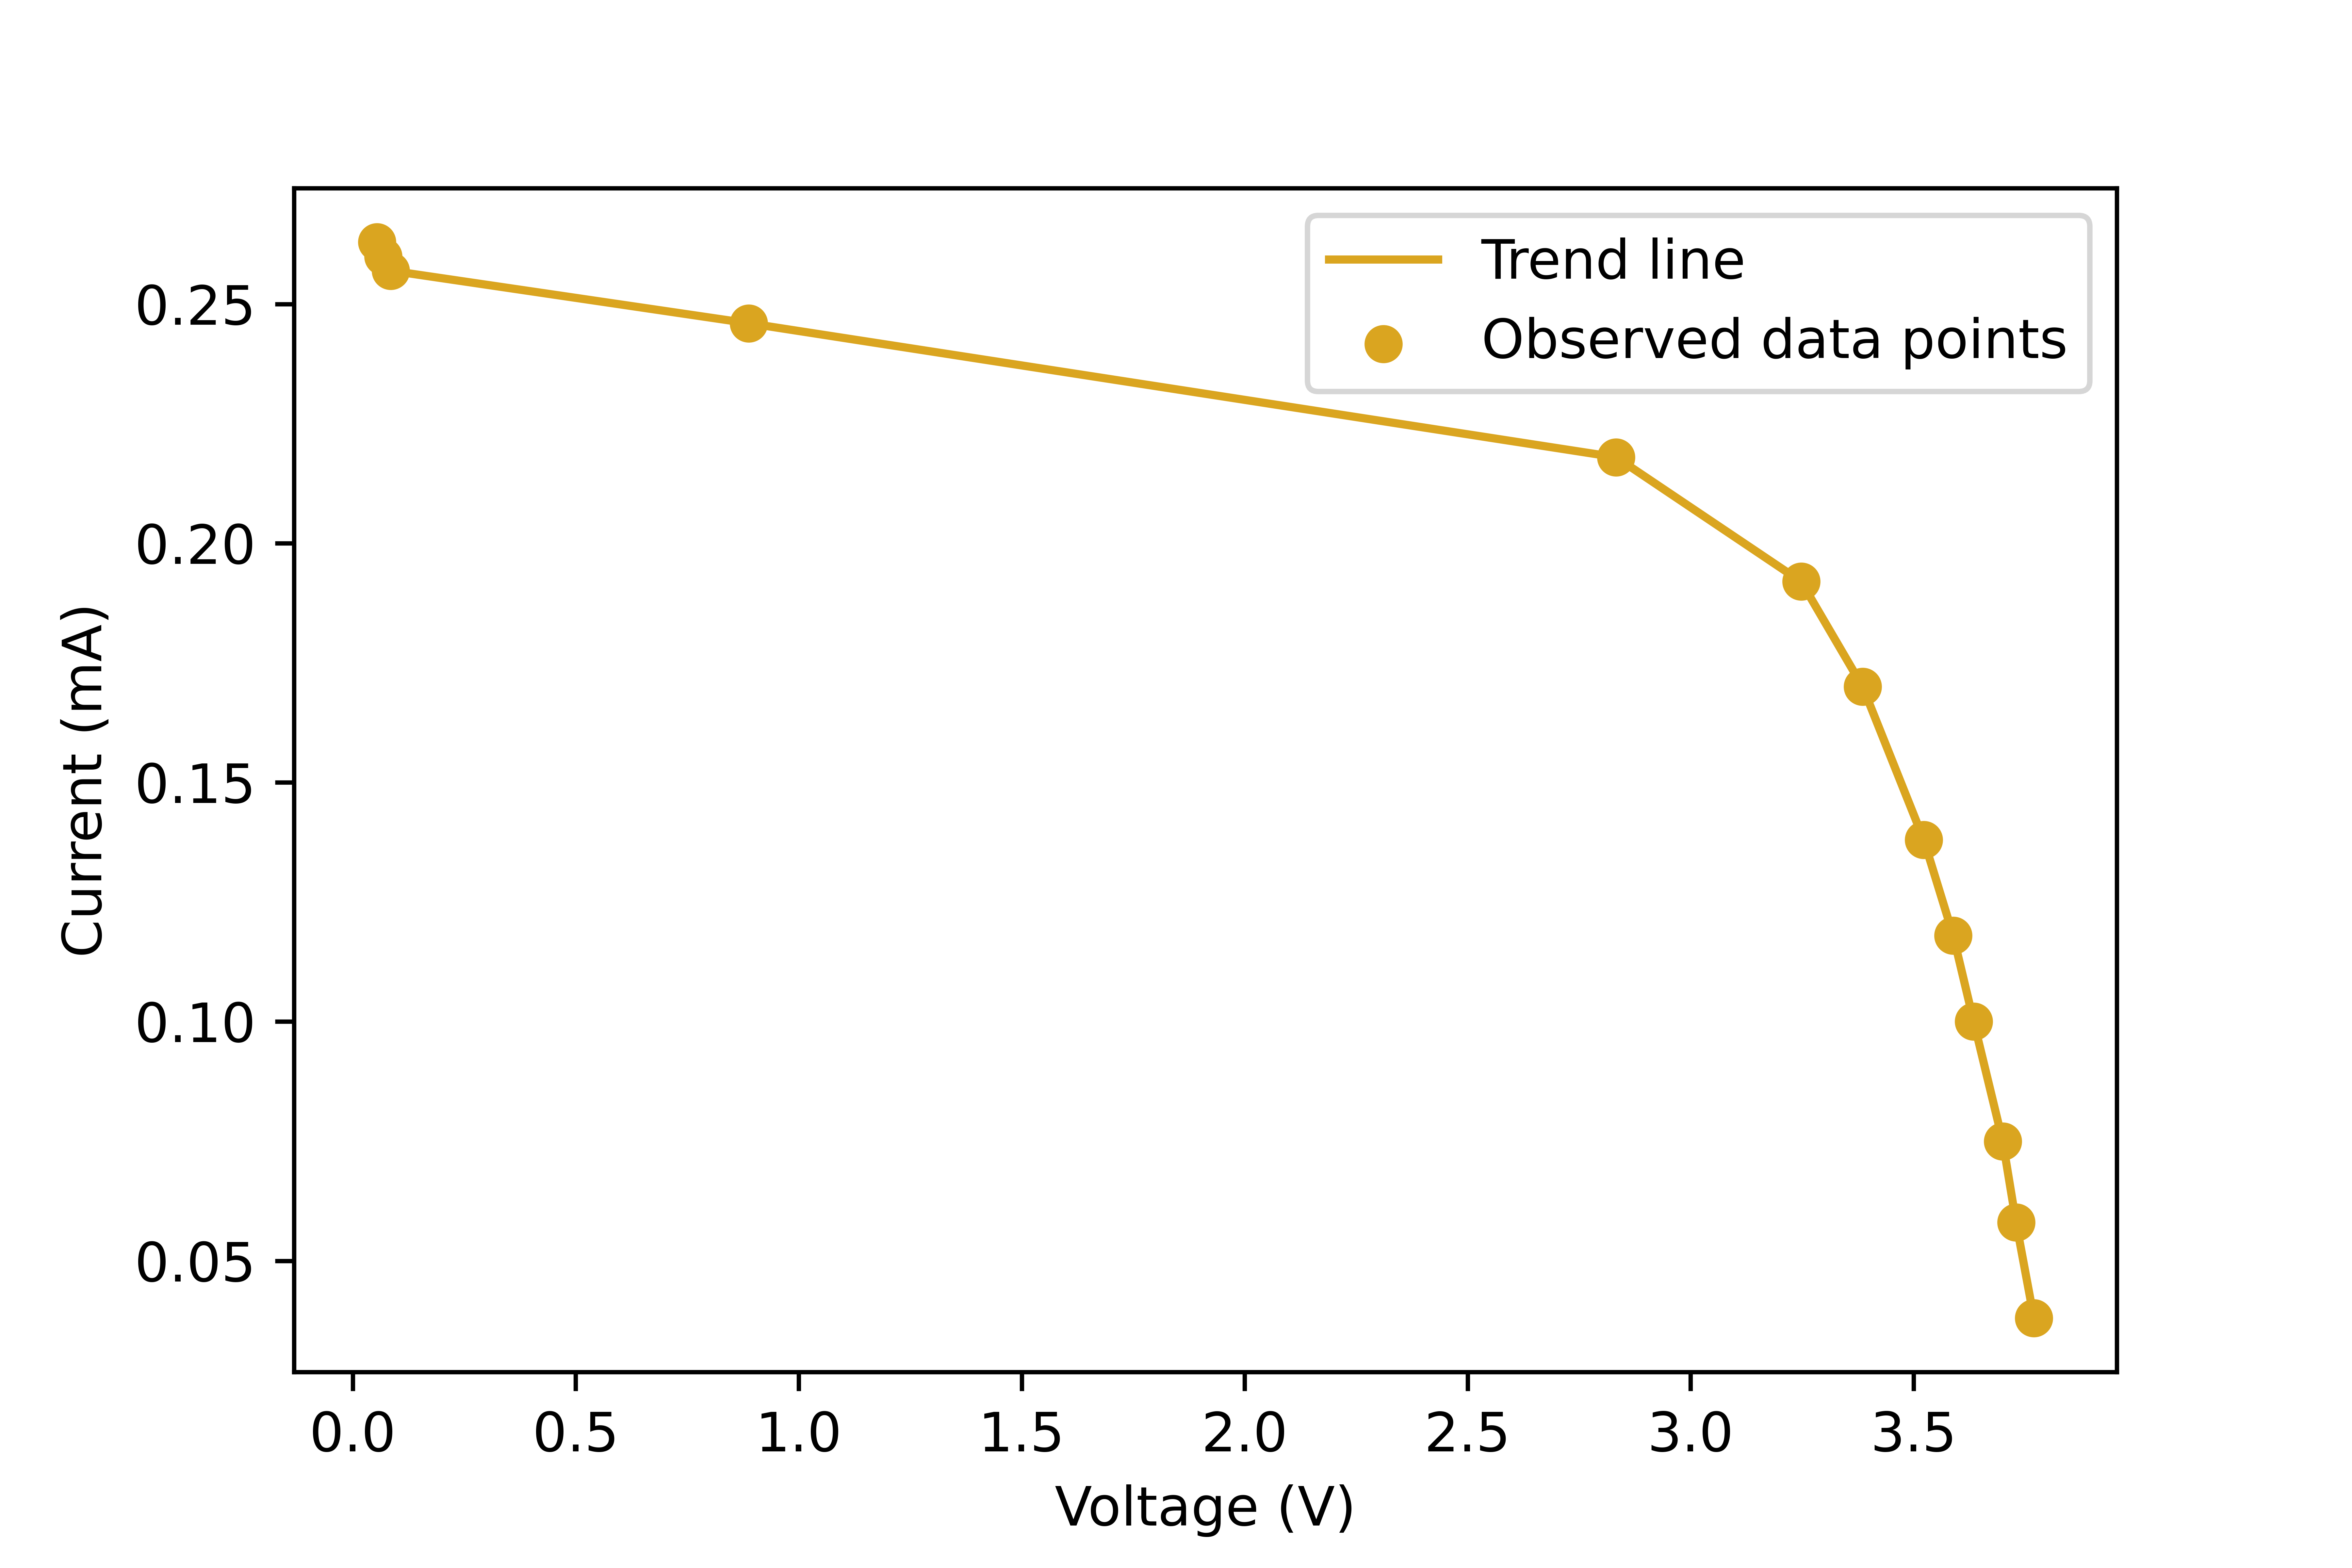
\includegraphics[scale = 0.54]{Figures/plot-iv-lamp-yellow.png}
            \caption{With yellow filter}
            \label{fig:iv-lamp-yellow}
        \end{subfigure}
        \hfill
        \begin{subfigure}[b]{0.49\textwidth}
            \centering
            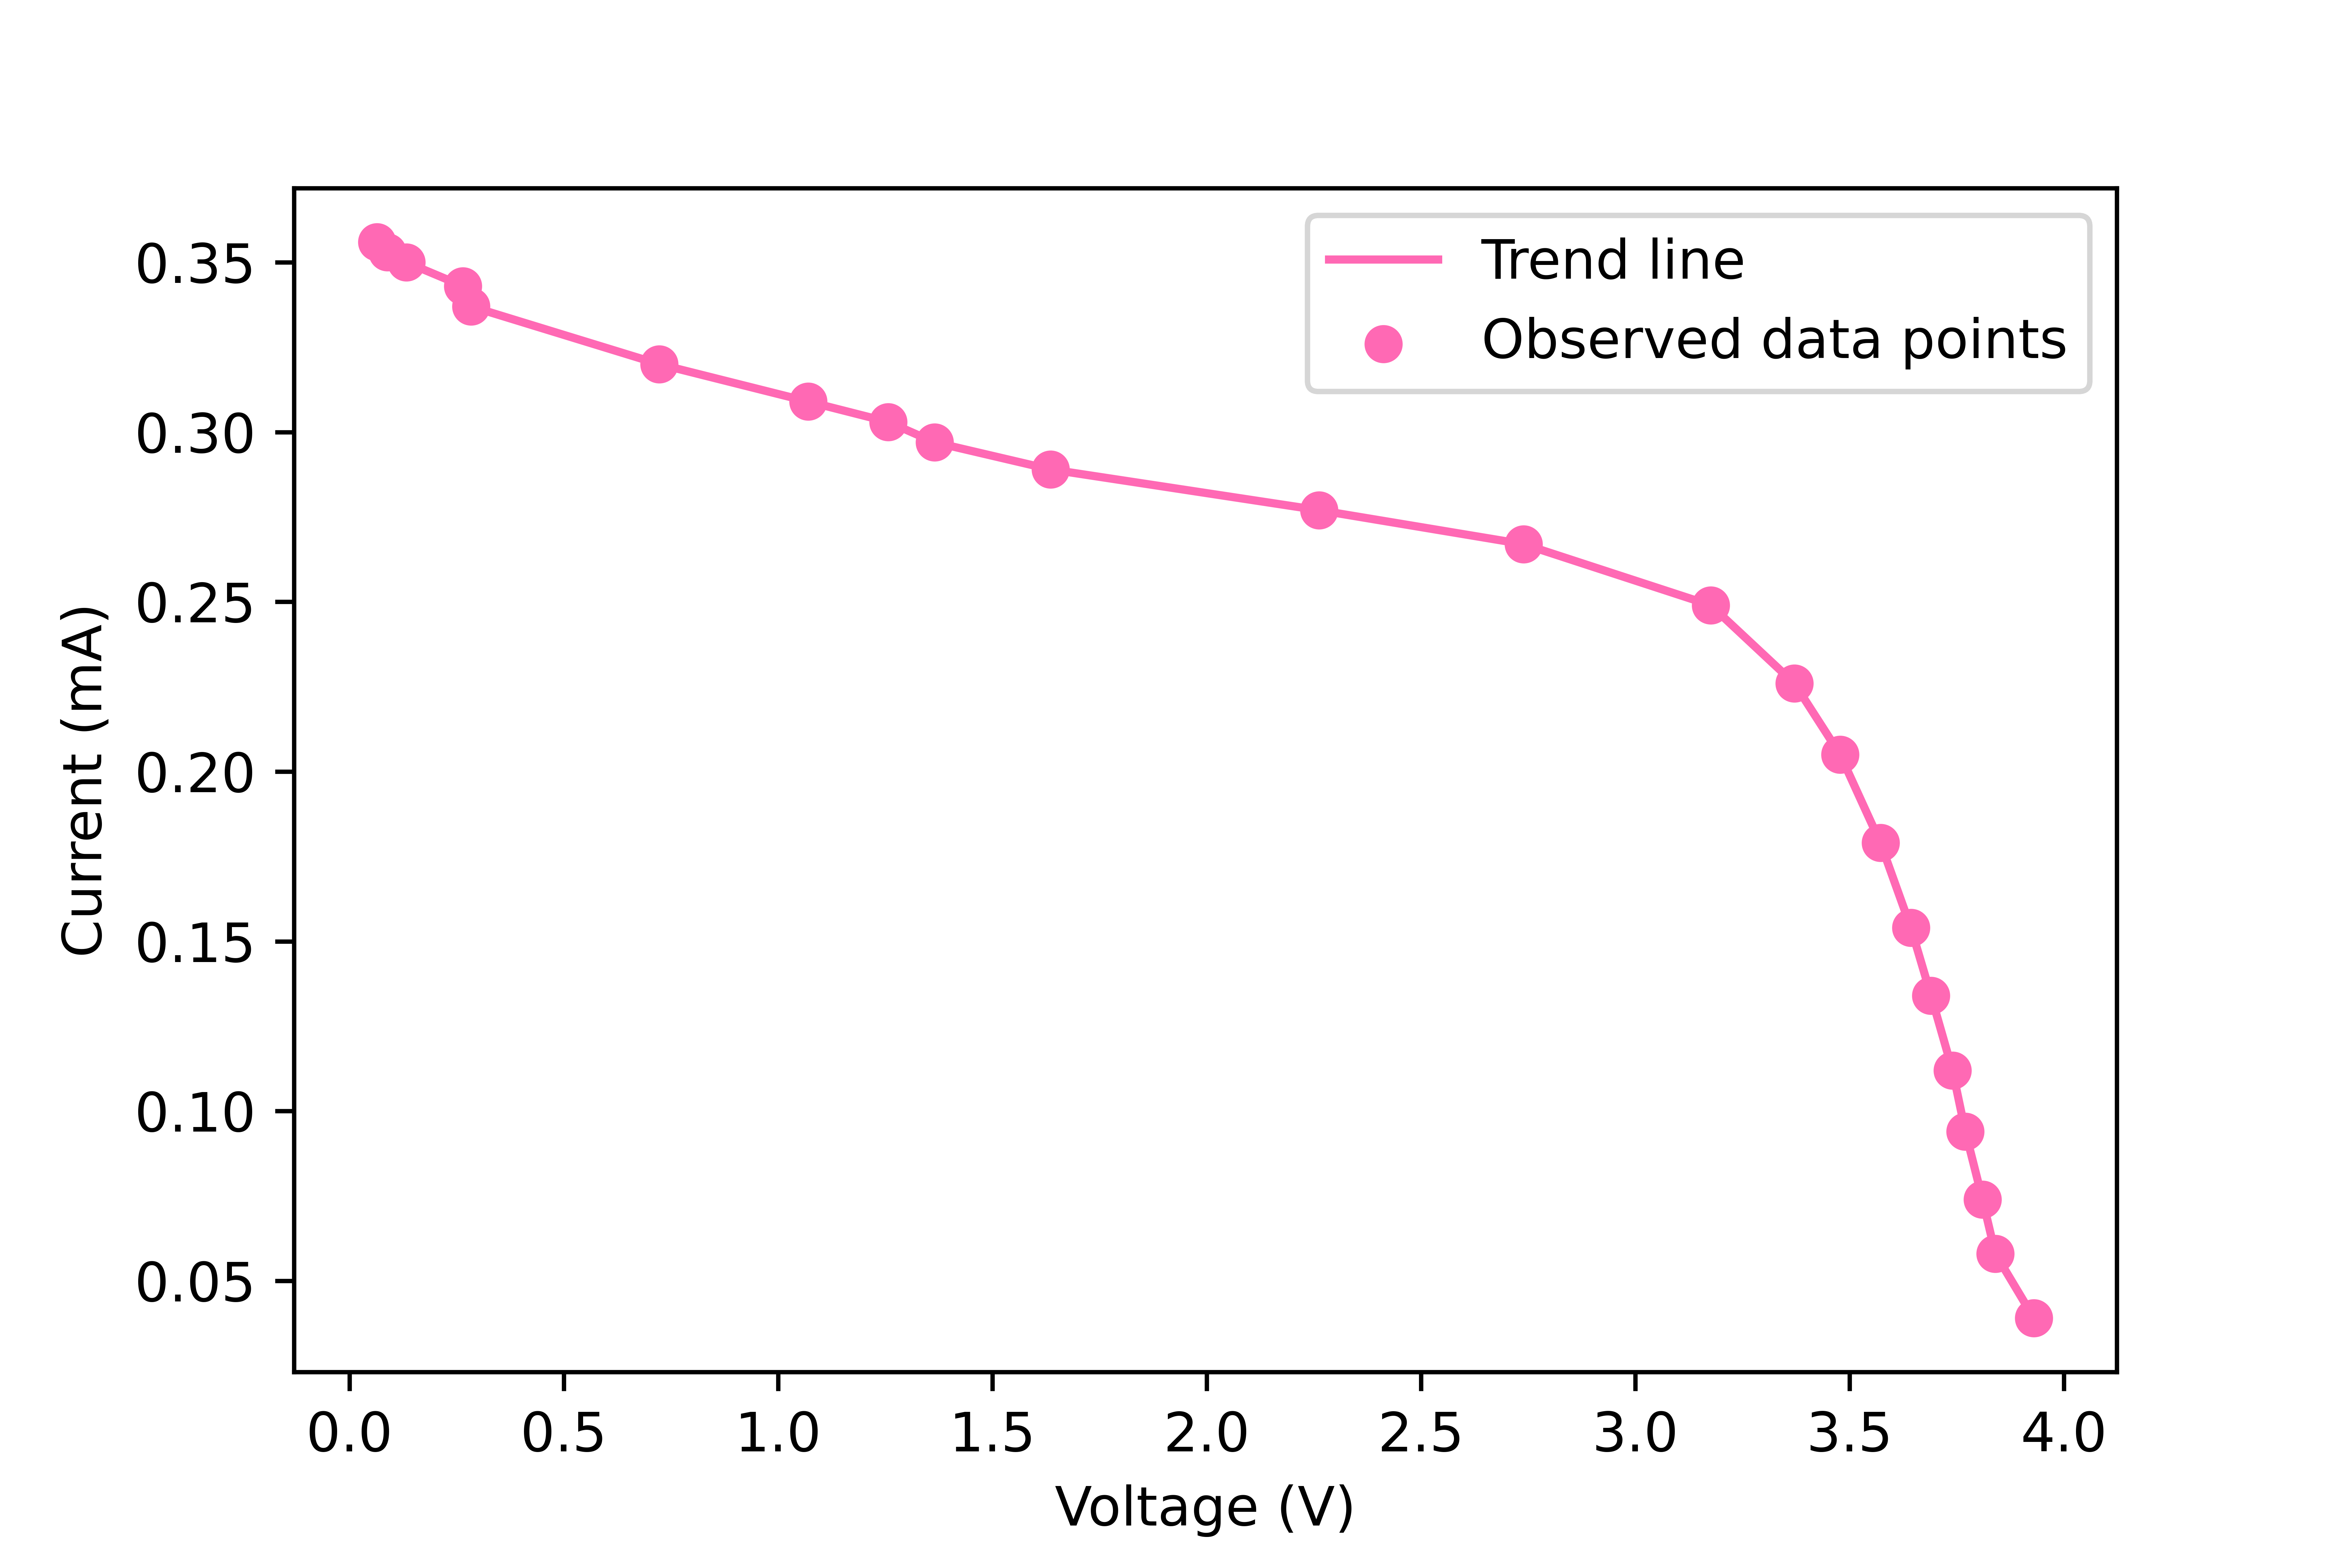
\includegraphics[scale = 0.54]{Figures/plot-iv-lamp-pink.png}
            \caption{With pink filter}
            \label{fig:iv-lamp-pink}
        \end{subfigure}
            \caption{I-V characteristic curve of solar cell illuminated by the incandescent halogen lamp with various filters}
            \label{fig:iv-lamp}
    \end{figure*}
    
    


    
    \begin{table*}[]
    \caption{I-V characterization of the solar cell illuminated by the sun with various filters}
    \label{tab:iv-sun}
    \setlength{\tabcolsep}{12pt}
    \begin{tabular}{@{}ccccccccccc@{}}
    \toprule
    \multicolumn{2}{c}{\textbf{No Filter}} &  & \multicolumn{2}{c}{\textbf{Red filter}} &  & \multicolumn{2}{c}{\textbf{Yellow filter}} &  & \multicolumn{2}{c}{\textbf{Pink filter}} \\ \cmidrule(r){1-2} \cmidrule(lr){4-5} \cmidrule(lr){7-8} \cmidrule(l){10-11} 
    \begin{tabular}[c]{@{}c@{}}\textit{Voltage}\\ ($\si{\volt}$)\end{tabular} & \begin{tabular}[c]{@{}c@{}}\textit{Current} \\ ($\si{\milli \ampere}$)\end{tabular} &  & \begin{tabular}[c]{@{}c@{}}\textit{Voltage}\\ ($\si{\volt}$)\end{tabular} & \begin{tabular}[c]{@{}c@{}}\textit{Current} \\ ($\si{\milli \ampere}$)\end{tabular} &  & \begin{tabular}[c]{@{}c@{}}\textit{Voltage}\\ ($\si{\volt}$)\end{tabular} & \begin{tabular}[c]{@{}c@{}}\textit{Current} \\ ($\si{\milli \ampere}$)\end{tabular} &  & \begin{tabular}[c]{@{}c@{}}\textit{Voltage}\\ ($\si{\volt}$)\end{tabular} & \begin{tabular}[c]{@{}c@{}}\textit{Current} \\ ($\si{\milli \ampere}$)\end{tabular} \\ \midrule
    6 & 0.05 &  & 5.67 & 0.05 &  & 5.73 & 0.06 &  & 5.78 & 0.06 \\
    5.96 & 0.41 &  & 5.67 & 1.77 &  & 5.71 & 0.12 &  & 5.76 & 0.35 \\
    5.92 & 0.98 &  & 5.6 & 7.76 &  & 5.71 & 0.26 &  & 5.73 & 2.74 \\
    5.91 & 1.1 &  & 5.56 & 10.32 &  & 5.7 & 0.86 &  & 5.67 & 7.33 \\
    5.9 & 2.17 &  & 5.4 & 21.26 &  & 5.61 & 8.83 &  & 5.64 & 9.82 \\
    \multirow{2}{*}{5.88} & \multirow{2}{*}{3.44} &  & \multirow{2}{*}{5.33} & \multirow{2}{*}{25.8} &  & 5.49 & 18.64 &  & 5.59 & 13.78 \\
     &  &  &  &  &  & 5.43 & 22.63 &  & 5.48 & 21.62 \\
    \multirow{2}{*}{5.78} & \multirow{2}{*}{11.98} &  & \multirow{2}{*}{5.26} & \multirow{2}{*}{29.06} &  & 5.26 & 32.33 &  & \multirow{2}{*}{5.35} & \multirow{2}{*}{29.86} \\
     &  &  &  &  &  & 5.18 & 36.69 &  &  &  \\
    \multirow{2}{*}{5.68} & \multirow{2}{*}{21.26} &  & \multirow{2}{*}{5.2} & \multirow{2}{*}{32.2} &  & 5.08 & 41.1 &  & 5.26 & 35.45 \\
     &  &  &  &  &  & 4.94 & 44.9 &  & 5.16 & 40.1 \\
    5.54 & 31.55 &  & 5.1 & 36.26 &  & 4.78 & 46.5 &  & 4.98 & 46.1 \\
    5.47 & 38.6 &  & 4.98 & 40.1 &  & 3.7 & 47.4 &  & 4.29 & 49.4 \\
    5.25 & 52.8 &  & 4.83 & 42.7 &  & 3 & 47.5 &  & 3.23 & 49.4 \\
    5.1 & 61.5 &  & 4.13 & 43 &  & 2.12 & 48.4 &  & 1.855 & 50.9 \\
    1.17 & 69.8 &  & 0.522 & 45.6 &  & 1.69 & 48.9 &  & 0.598 & 52.5 \\
    1.1 & 70.1 &  & 0.452 & 45.9 &  & 0.28 & 51.1 &  & 0.454 & 52.9 \\ \bottomrule
    \end{tabular}
    \end{table*}
    
    \begin{figure*}
        \centering
        \begin{subfigure}[b]{0.49\textwidth}
            \centering
            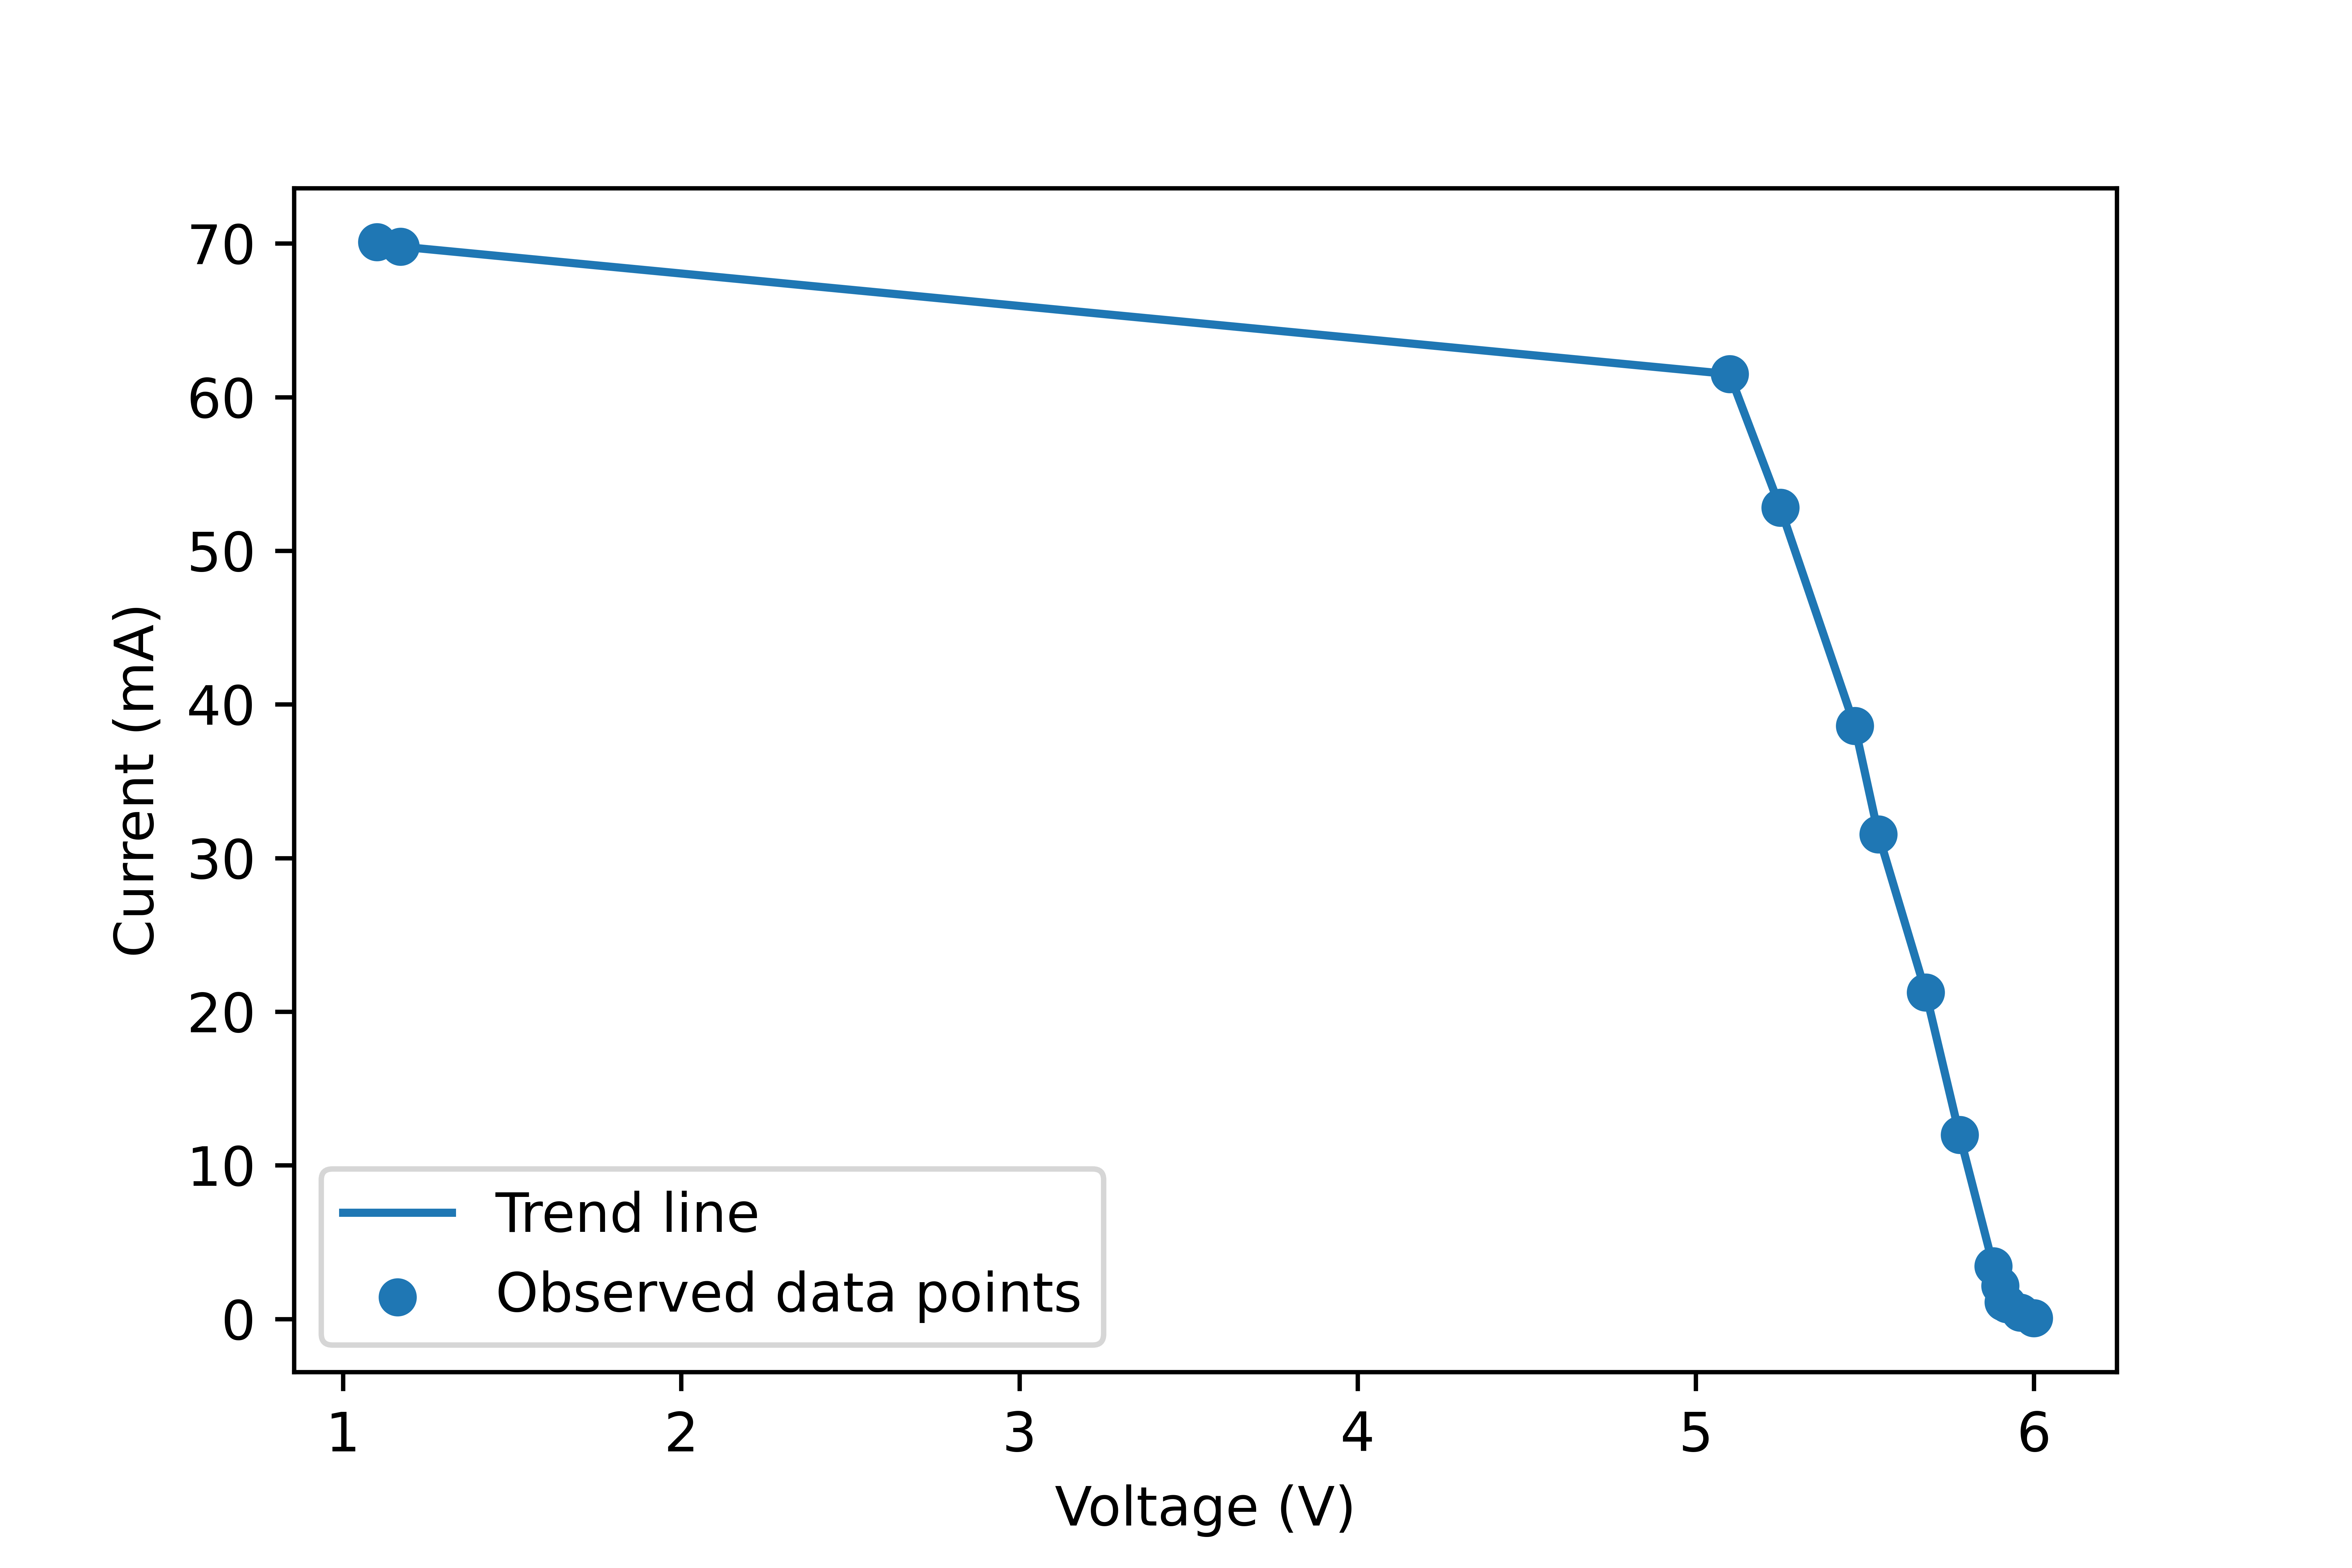
\includegraphics[scale = 0.54]{Figures/plot-iv-sun-nofilter.png}
            \caption{With no filter}
            \label{fig:iv-sun-nofilter}
        \end{subfigure}
        \hfill
        \begin{subfigure}[b]{0.49\textwidth}
            \centering
            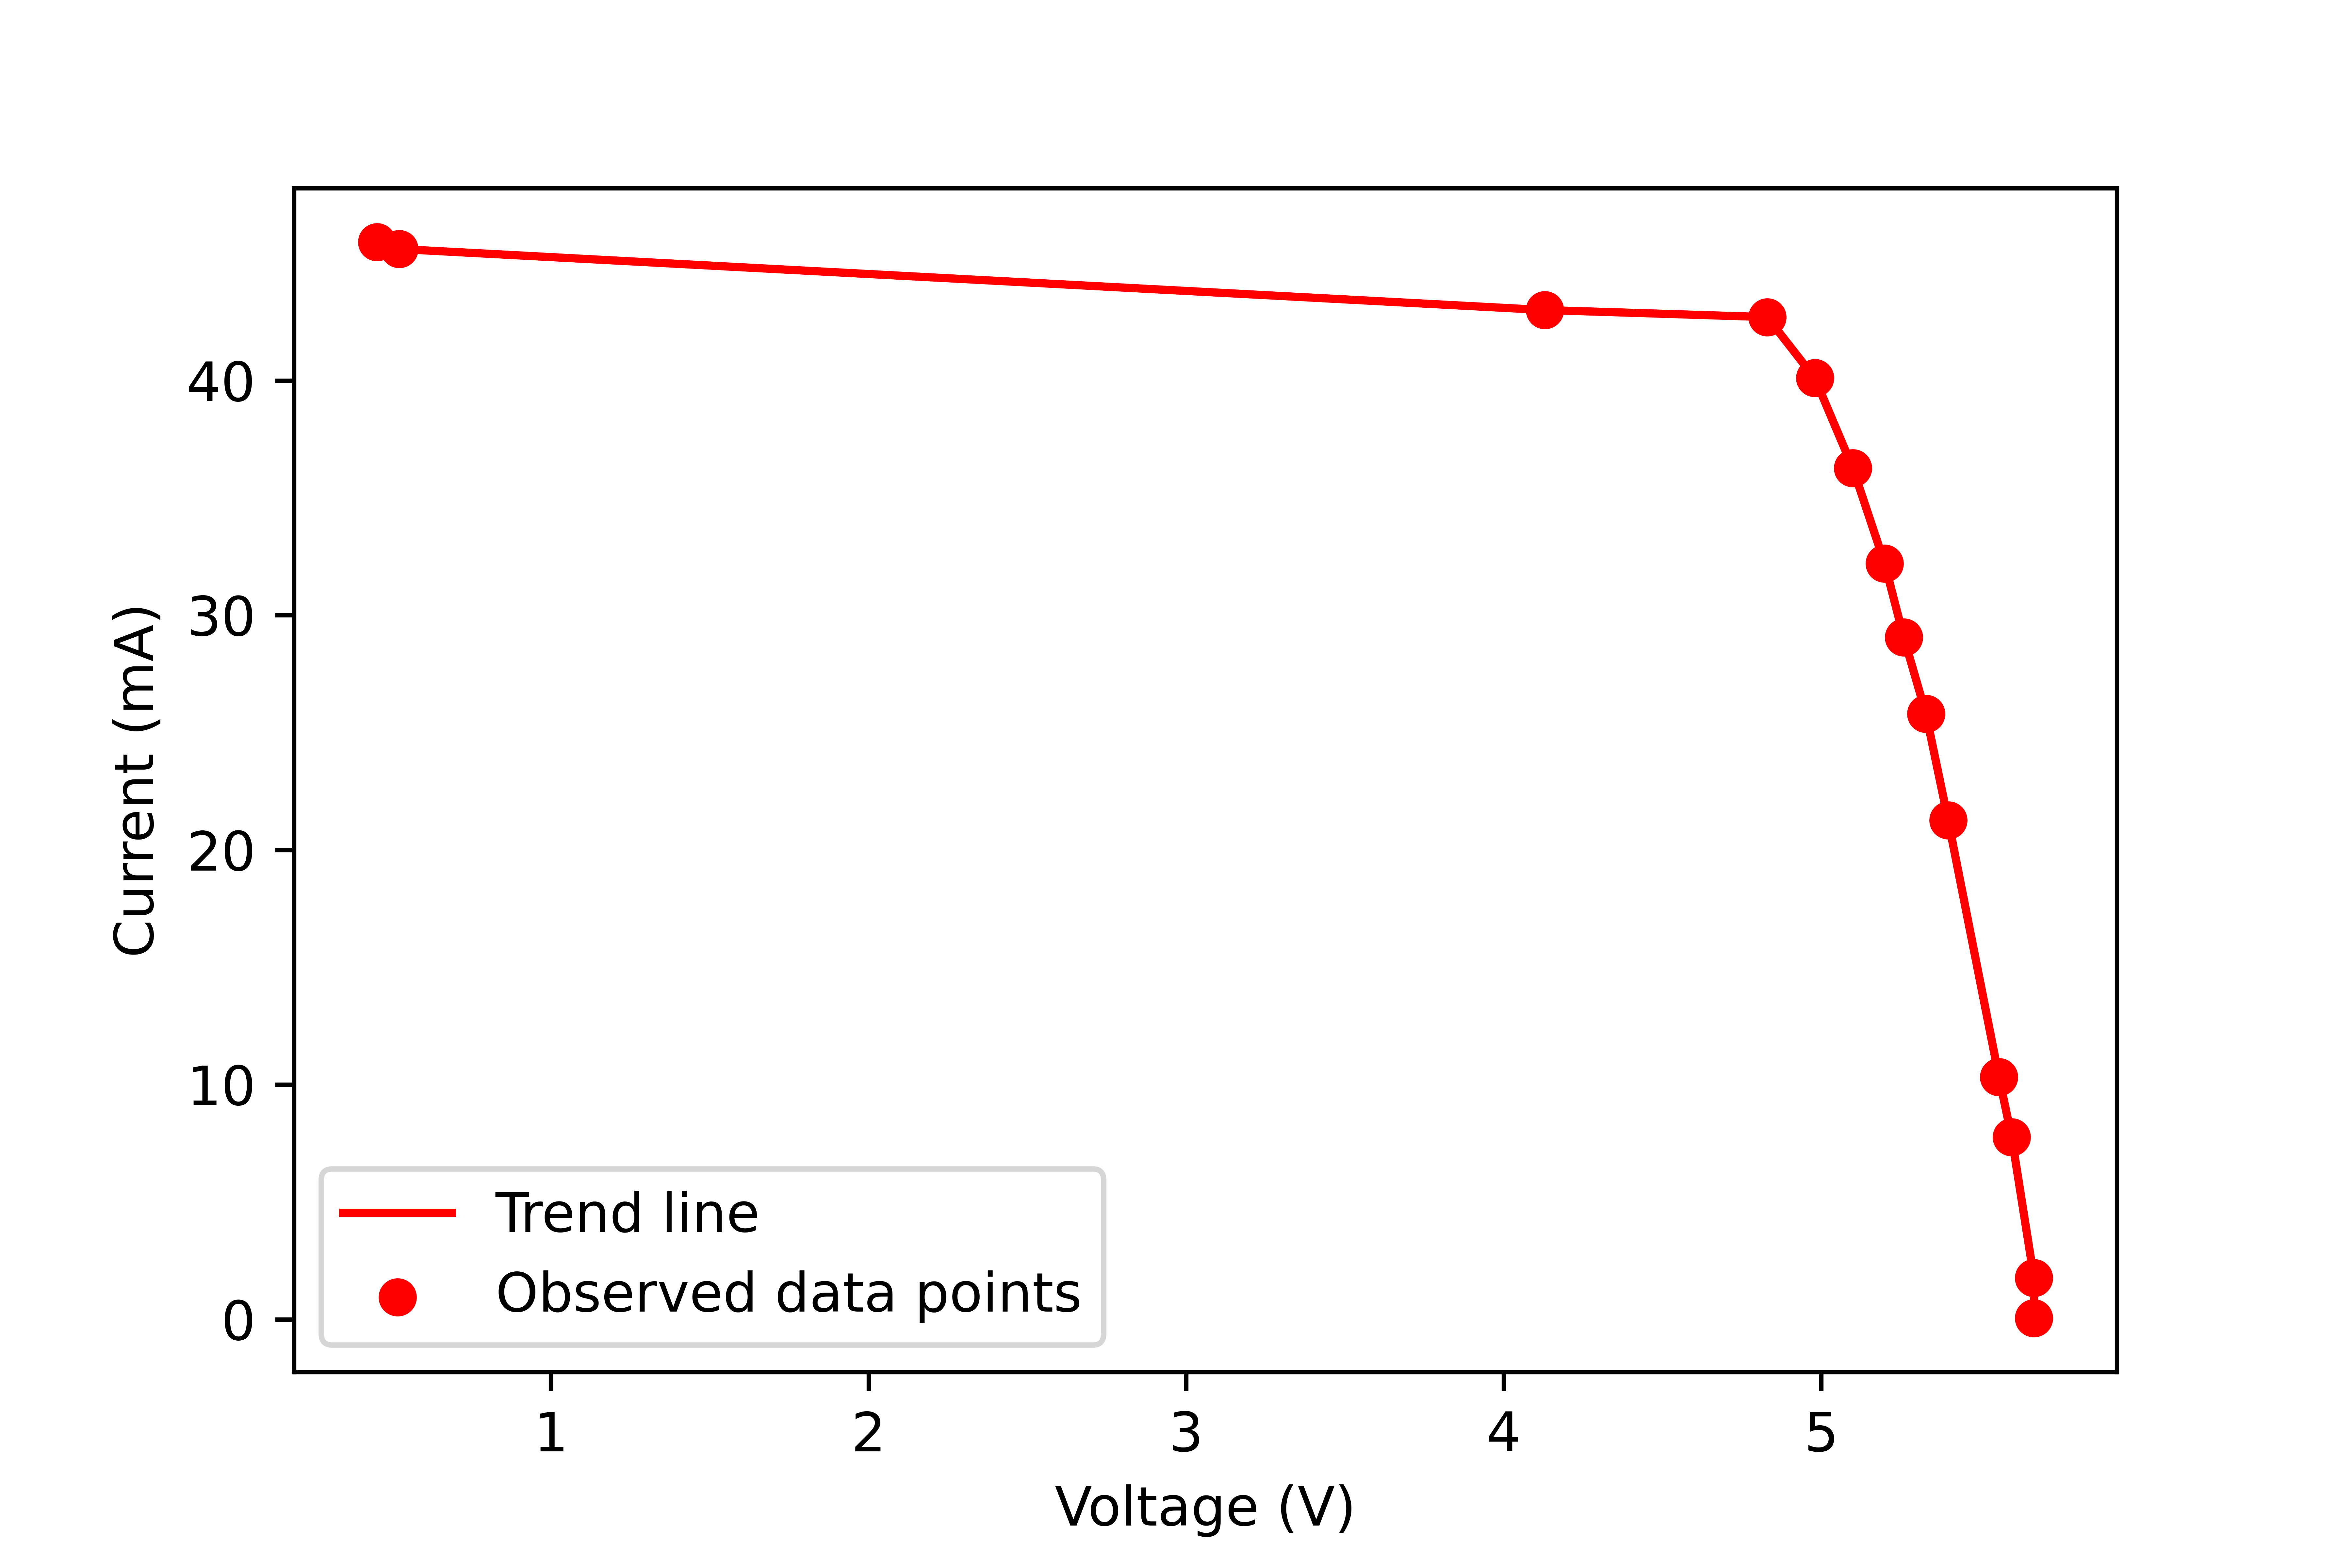
\includegraphics[scale = 0.54]{Figures/plot-iv-sun-red.png}
            \caption{With red filter}
            \label{fig:iv-sun-red}
        \end{subfigure}
        \hfill
        \begin{subfigure}[b]{0.49\textwidth}
            \centering
            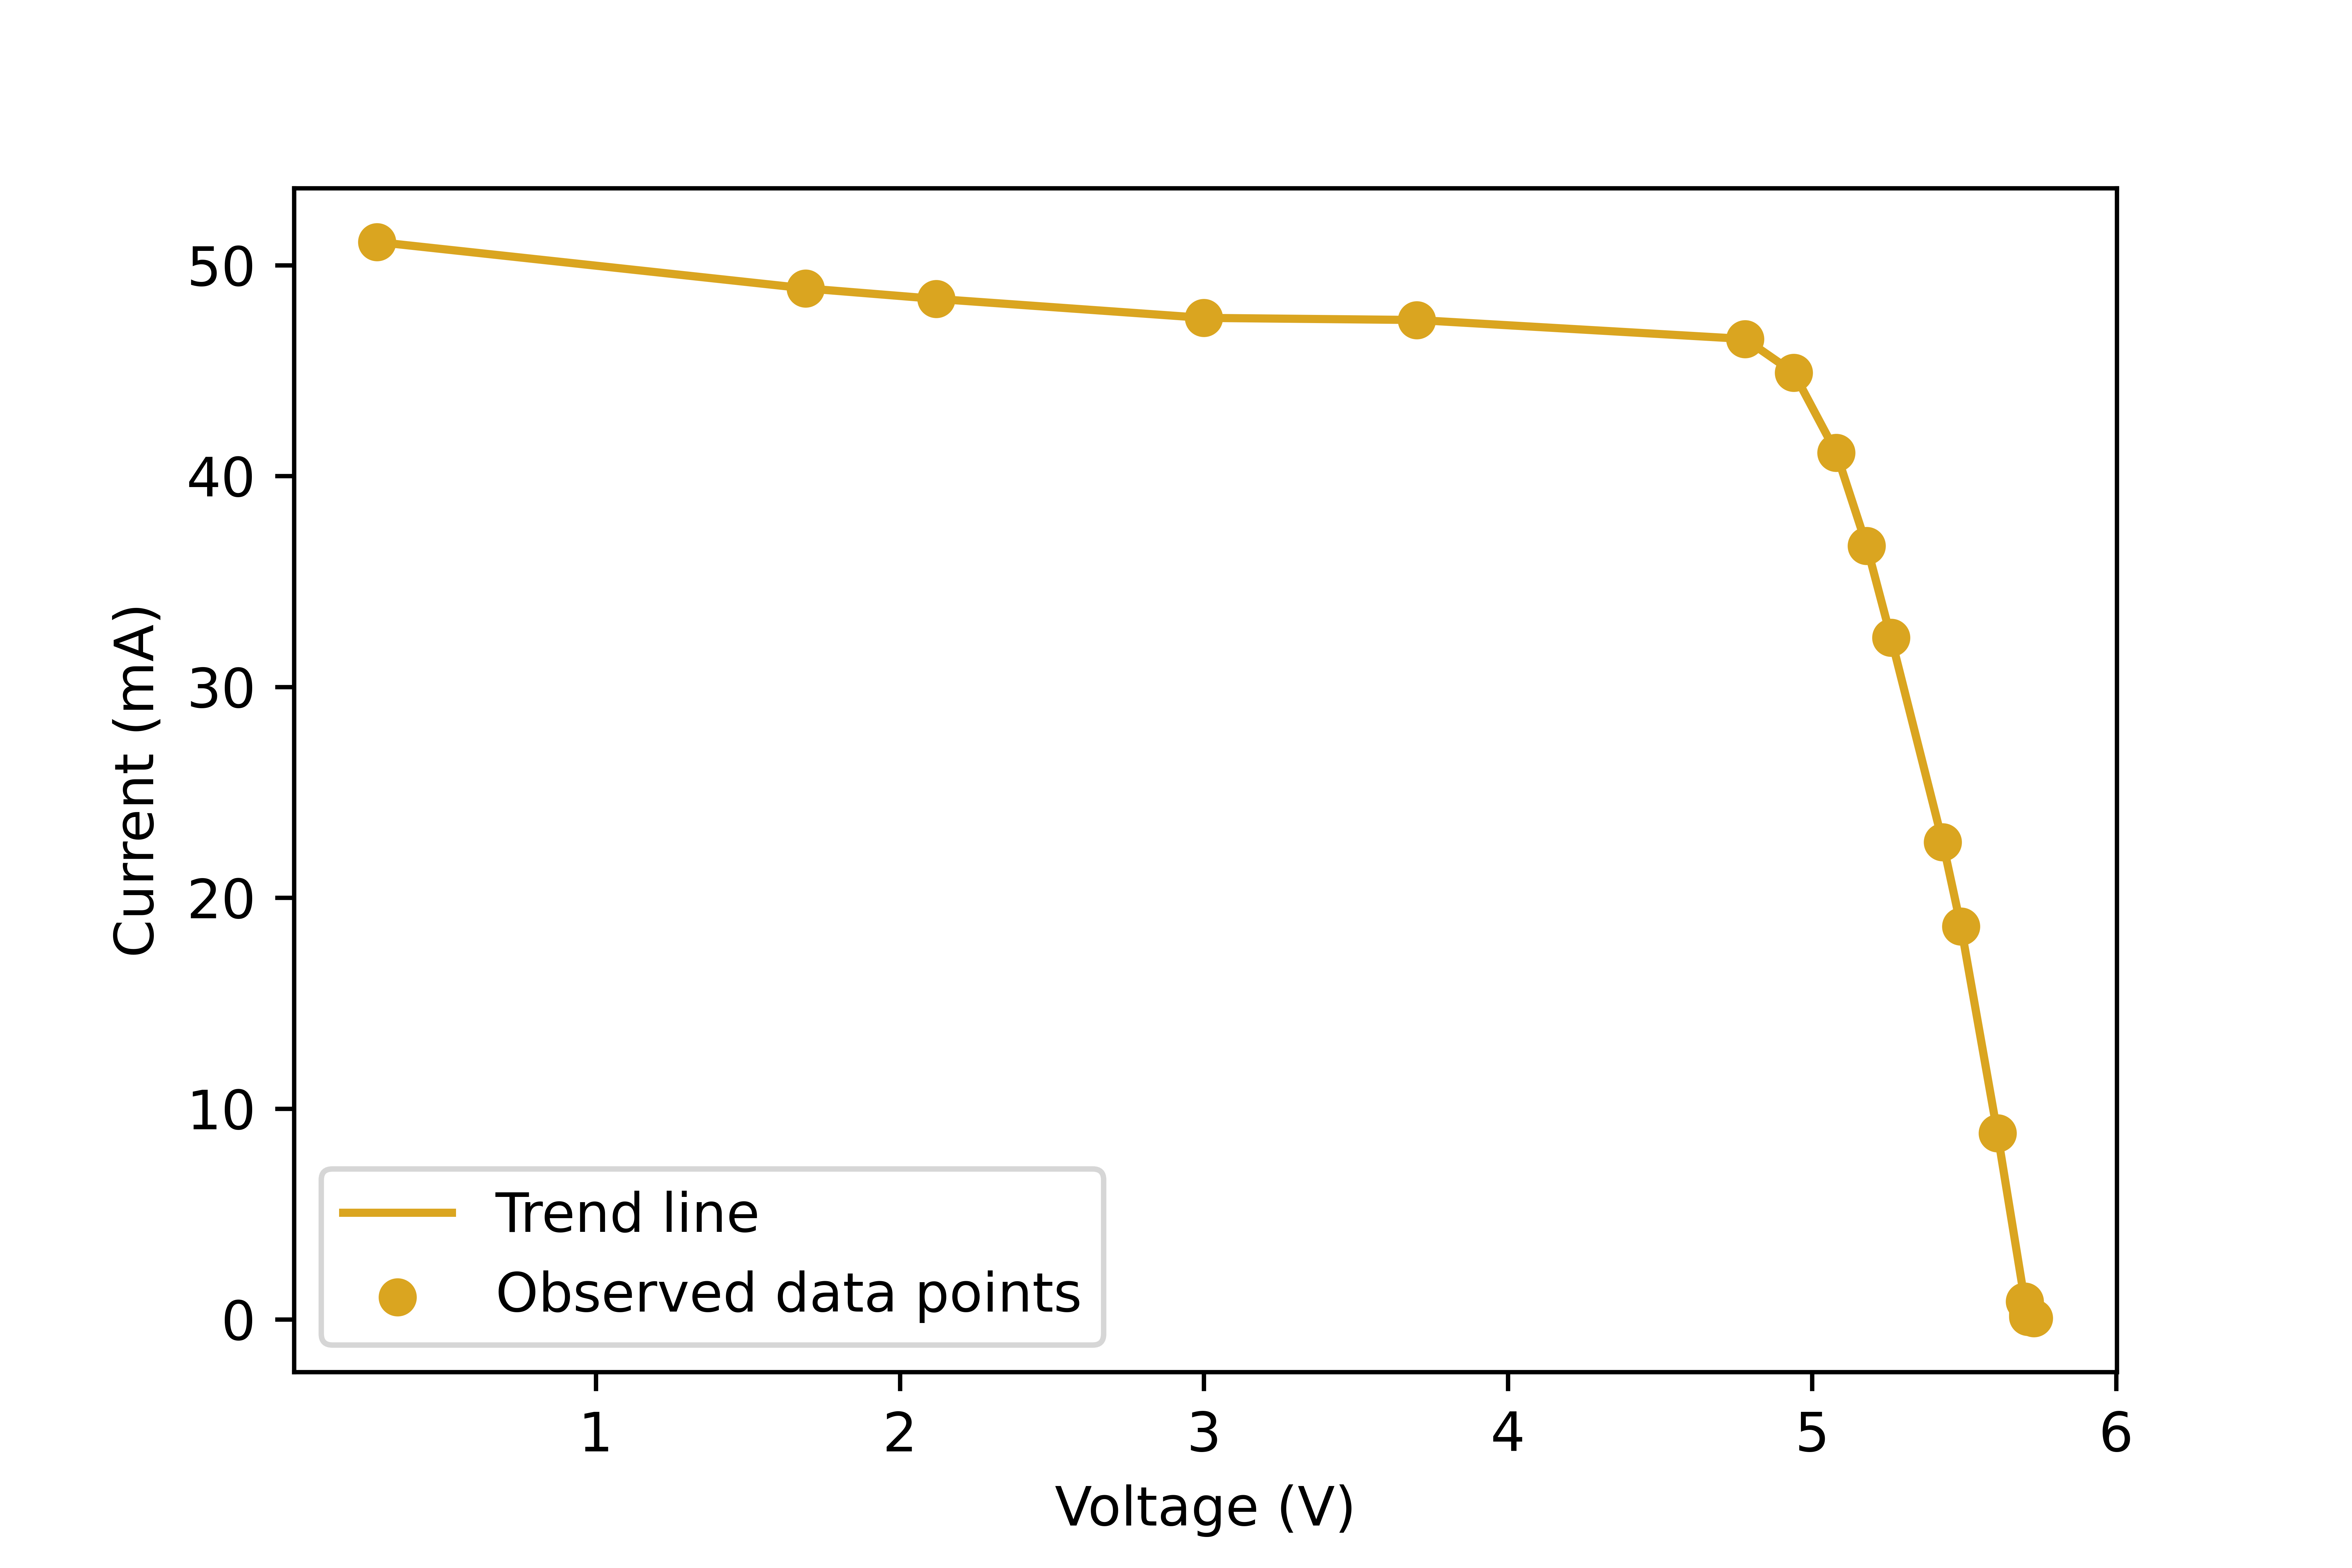
\includegraphics[scale = 0.54]{Figures/plot-iv-sun-yellow.png}
            \caption{With yellow filter}
            \label{fig:iv-sun-yellow}
        \end{subfigure}
        \hfill
        \begin{subfigure}[b]{0.49\textwidth}
            \centering
            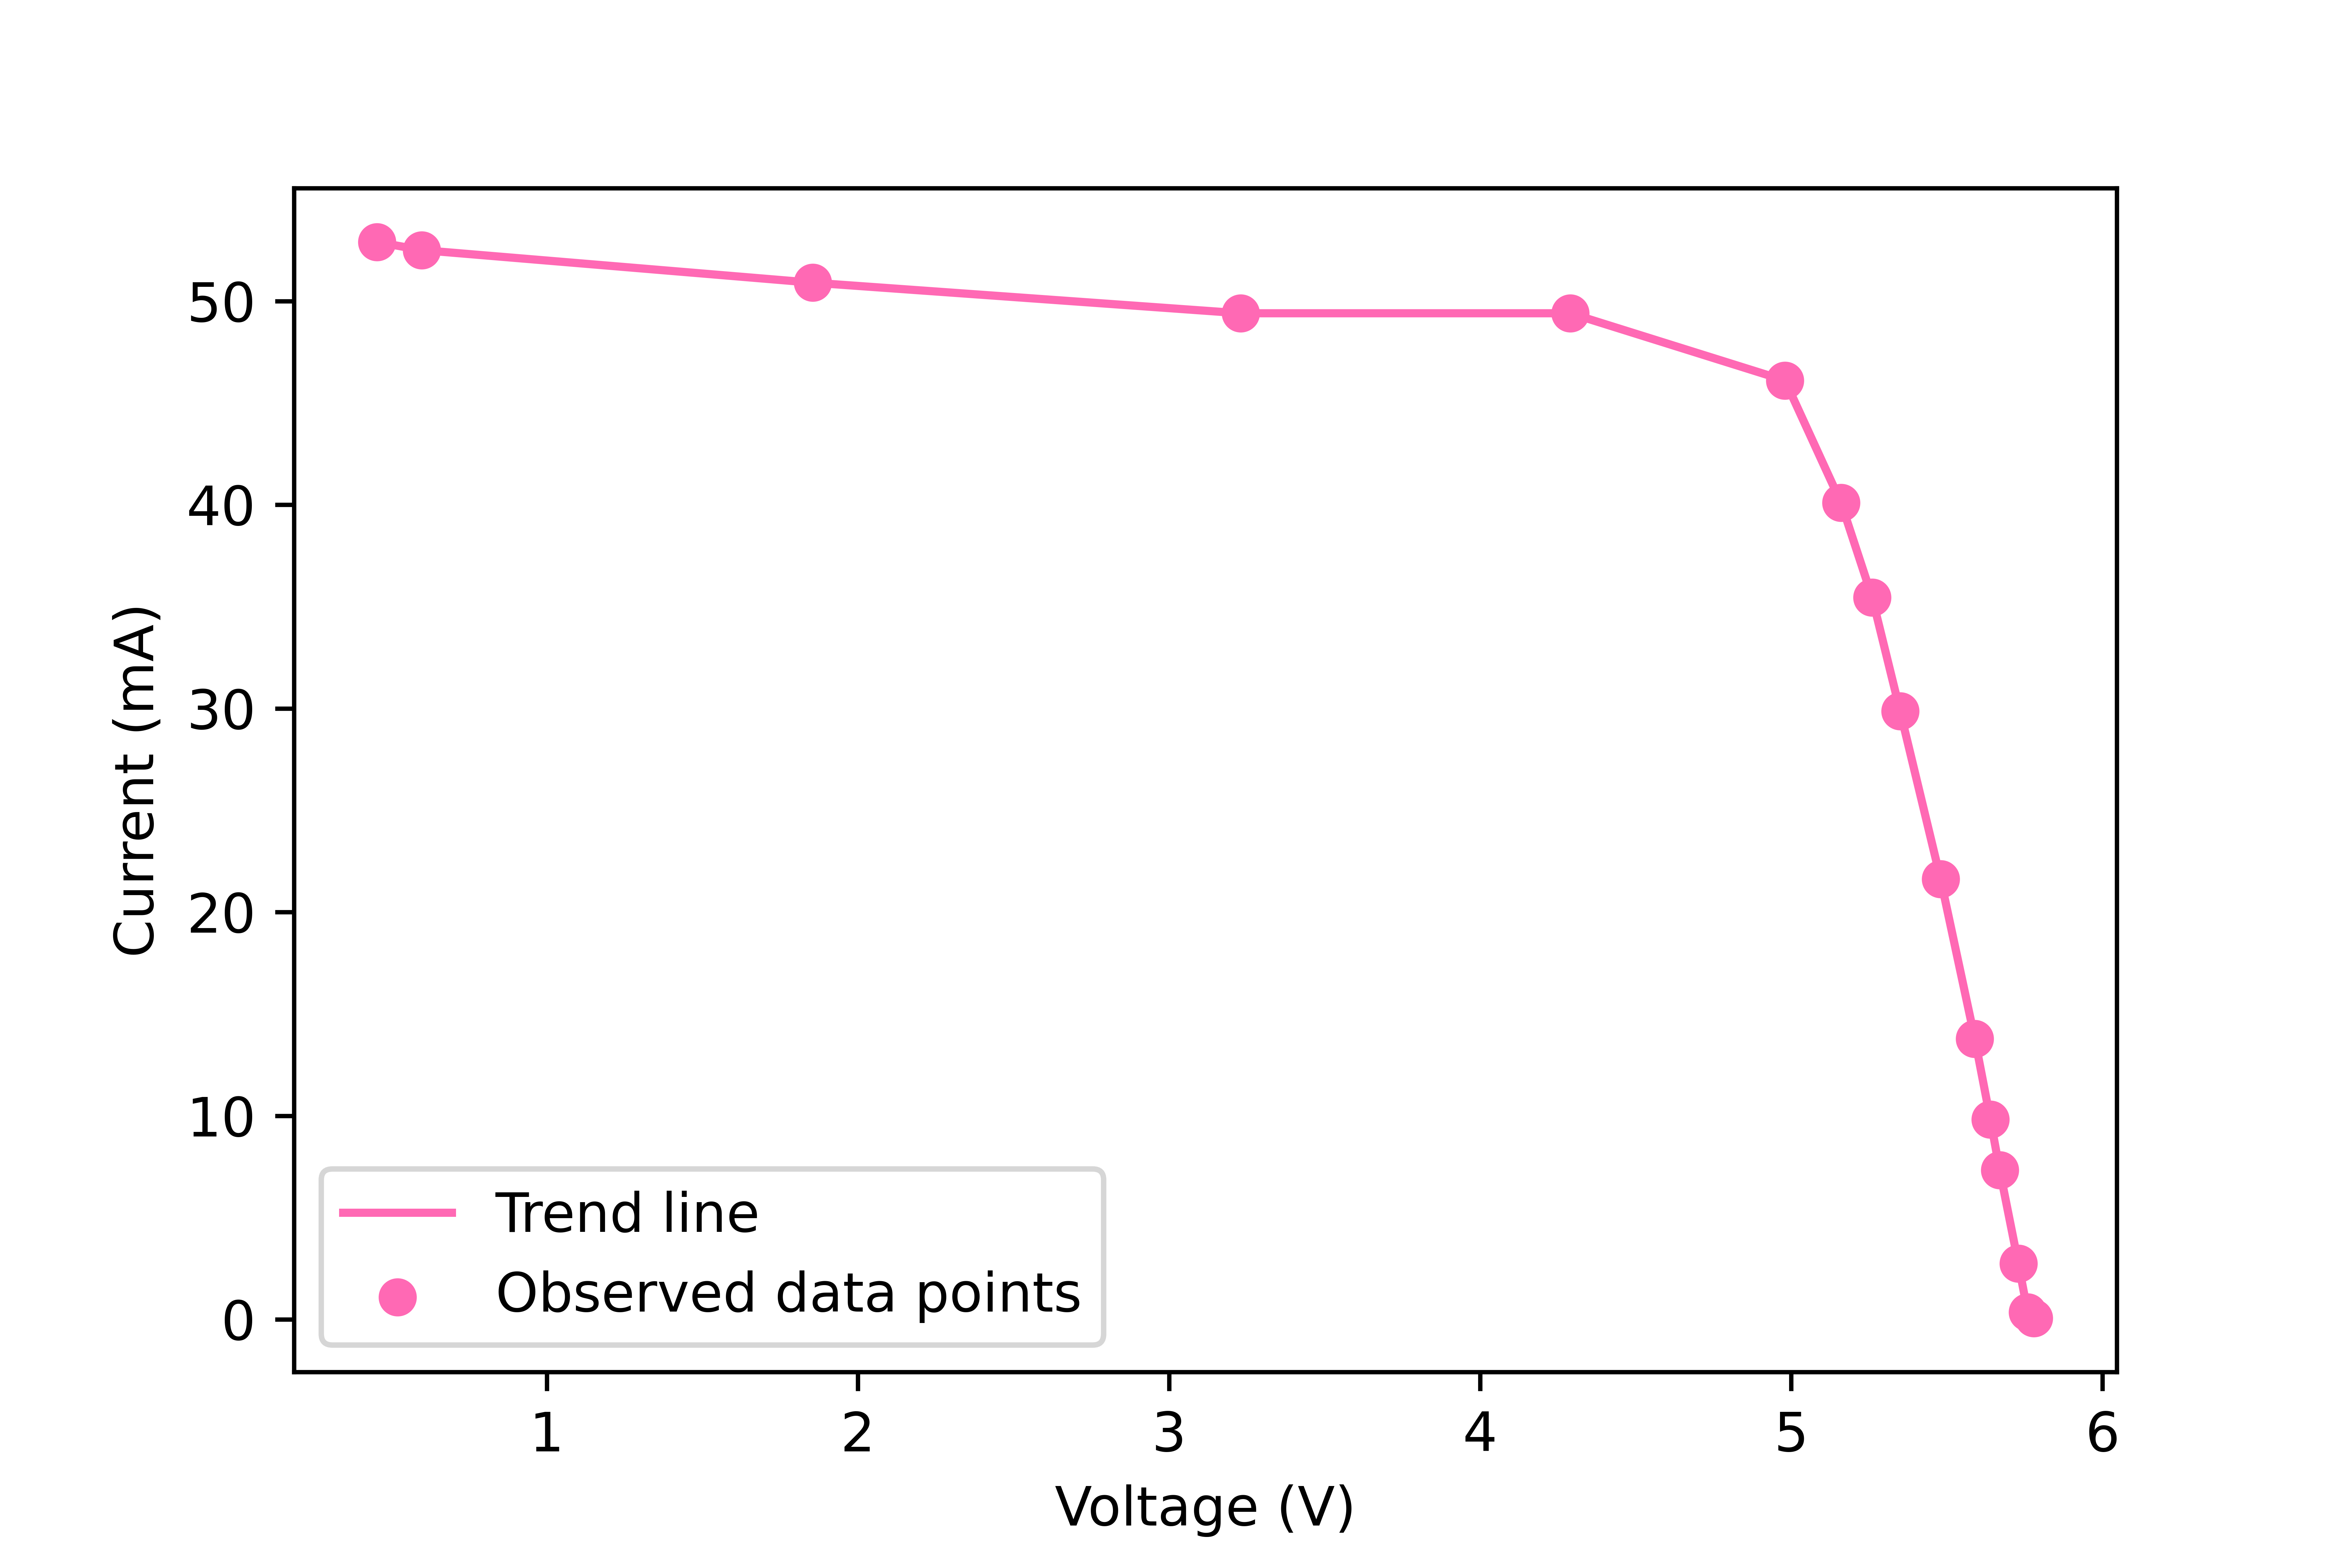
\includegraphics[scale = 0.54]{Figures/plot-iv-sun-pink.png}
            \caption{With pink filter}
            \label{fig:iv-sun-pink}
        \end{subfigure}
            \caption{I-V characteristic curve of solar cell illuminated by the sun with various filters}
            \label{fig:iv-sun}
    \end{figure*}

    
    
    
    \begin{table}[]
    \caption{C-V characterization of the solar cell under light conditions}
    \label{tab:cv-light}
    \setlength{\tabcolsep}{15pt}
    \begin{tabular}{@{}ccccc@{}}
    \toprule
    \begin{tabular}[c]{@{}c@{}}$\mathbf{V_{DC}}$\\ ($\si{\volt}$)\end{tabular} & \begin{tabular}[c]{@{}c@{}}$\mathbf{V_{DUT}}$\\ ($\si{\volt}$)\end{tabular} & \begin{tabular}[c]{@{}c@{}}$\mathbf{V_{OUT}}$\\ ($\si{\volt}$)\end{tabular} & \begin{tabular}[c]{@{}c@{}}$\mathbf{C_{DUT}}$\\ ($\si{\micro \farad}$)\end{tabular} & \begin{tabular}[c]{@{}c@{}}$\mathbf{1/C^2}$\\ ($\si{\per \micro \farad \squared}$)\end{tabular} \\ \midrule
    0.3 & -0.336 & 9.73 & 0.272 & 5.000 \\
    0.4 & -0.397 & 9.78 & 0.231 & 18.721 \\
    0.5 & -0.543 & 9.83 & 0.170 & 34.668 \\
    0.6 & -0.657 & 9.82 & 0.140 & 50.855 \\
    0.7 & -0.783 & 9.91 & 0.119 & 70.926 \\
    0.8 & -0.822 & 9.9 & 0.113 & 78.326 \\
    0.9 & -0.936 & 10.01 & 0.100 & 99.338 \\
    1 & -1.004 & 9.98 & 0.093 & 114.984 \\
    1.1 & -1.069 & 10 & 0.088 & 129.833 \\
    1.2 & -1.218 & 10.03 & 0.077 & 167.542 \\
    1.3 & -1.32 & 10.03 & 0.071 & 196.778 \\
    1.4 & -1.399 & 10.04 & 0.067 & 220.596 \\
    1.5 & -1.494 & 10.07 & 0.063 & 250.076 \\
    1.6 & -1.598 & 10.06 & 0.059 & 286.674 \\
    1.7 & -1.69 & 10.08 & 0.056 & 319.361 \\
    1.8 & -1.81 & 10.06 & 0.052 & 367.783 \\
    1.9 & -1.903 & 10.06 & 0.050 & 406.548 \\
    2 & -1.993 & 10.1 & 0.048 & 442.386 \\ \bottomrule
    \end{tabular}
    \end{table}
    
    \begin{figure}
        \centering
        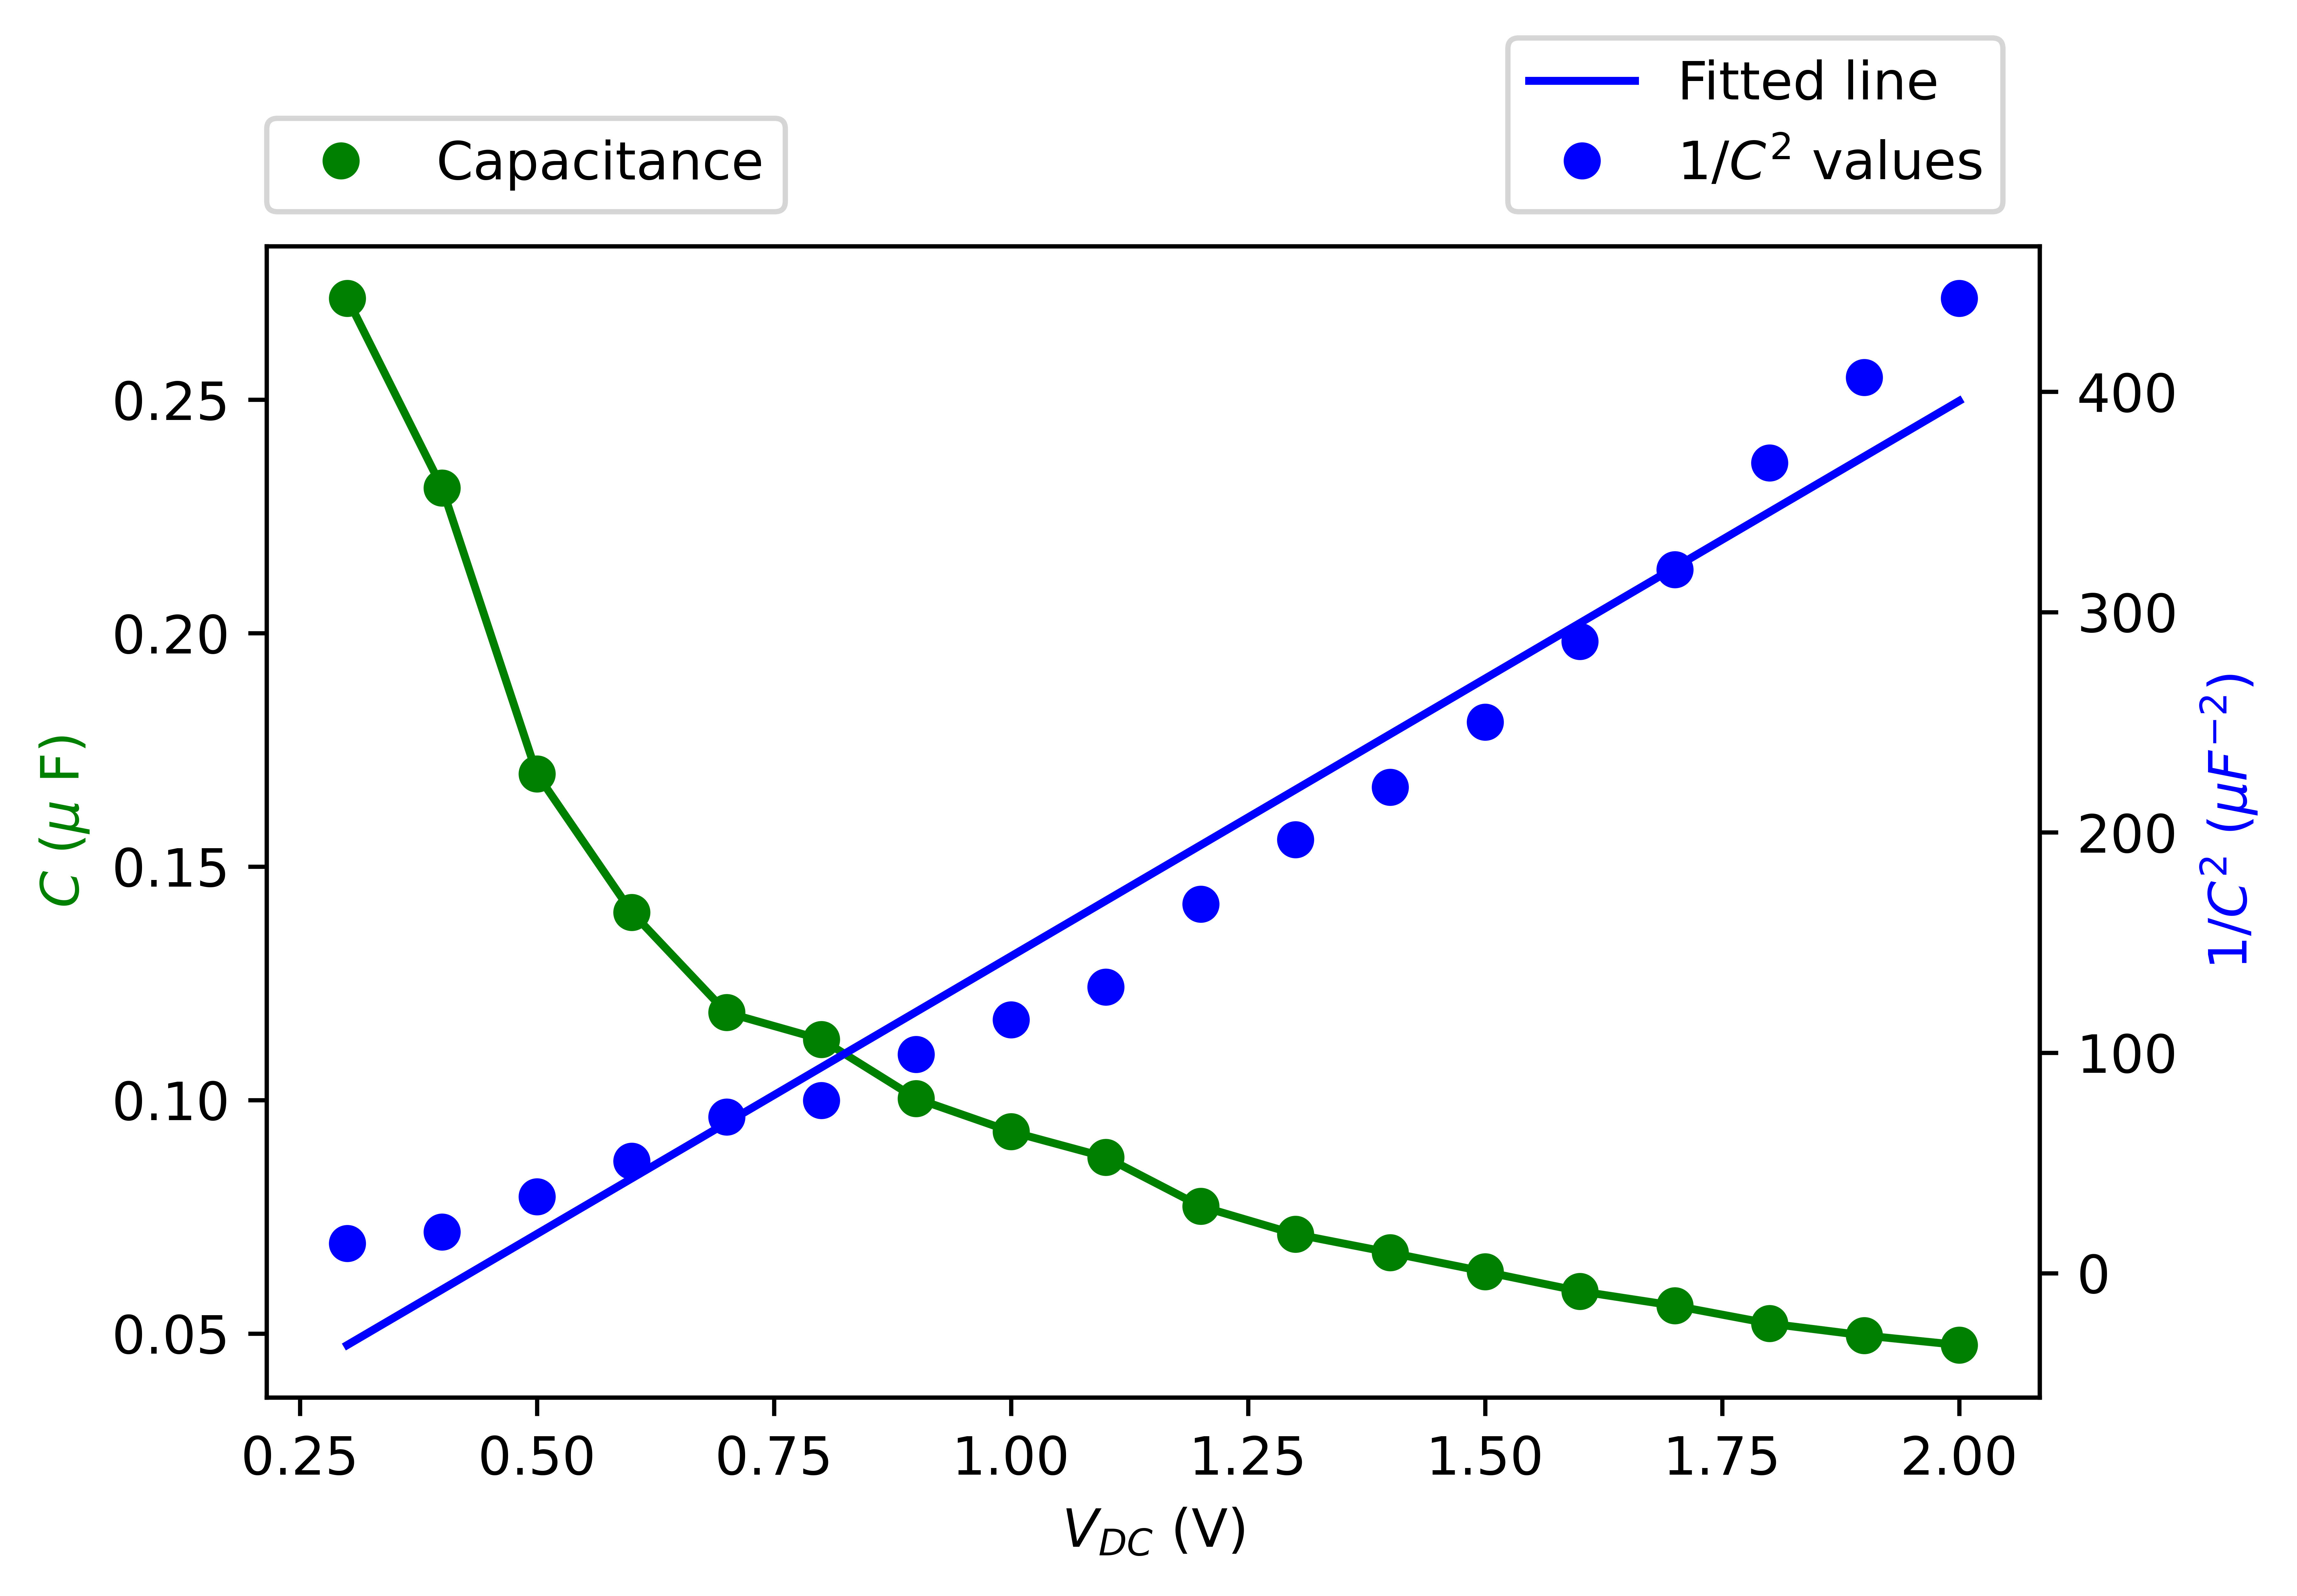
\includegraphics[scale = 0.54]{Figures/plot-cv-light.png}
        \caption{C-V characteristic curve for the solar cell under light conditions}
        \label{fig:cv-light}
    \end{figure}
    
    \begin{table}[]
    \caption{C-V characterization of the solar cell under dark conditions}
    \label{tab:cv-dark}
    \setlength{\tabcolsep}{15pt}
    \begin{tabular}{@{}ccccc@{}}
    \toprule
    \begin{tabular}[c]{@{}c@{}}$\mathbf{V_{DC}}$\\ ($\si{\volt}$)\end{tabular} & \begin{tabular}[c]{@{}c@{}}$\mathbf{V_{DUT}}$\\ ($\si{\volt}$)\end{tabular} & \begin{tabular}[c]{@{}c@{}}$\mathbf{V_{OUT}}$\\ ($\si{\volt}$)\end{tabular} & \begin{tabular}[c]{@{}c@{}}$\mathbf{C_{DUT}}$\\ ($\si{\nano \farad}$)\end{tabular} & \begin{tabular}[c]{@{}c@{}}$\mathbf{1/C^2}$\\ ($\si{\per \nano \farad \squared}$)\end{tabular} \\ \midrule
    0.3 & -0.346 & 0.019 & 0.515 & 3.768 \\
    0.4 & -0.485 & 0.024 & 0.464 & 4.640 \\
    0.5 & -0.564 & 0.027 & 0.449 & 4.957 \\
    0.6 & -0.666 & 0.032 & 0.451 & 4.921 \\
    0.7 & -0.762 & 0.036 & 0.443 & 5.090 \\
    0.8 & -0.843 & 0.039 & 0.434 & 5.308 \\
    0.9 & -0.943 & 0.044 & 0.438 & 5.219 \\
    1 & -1.055 & 0.045 & 0.400 & 6.245 \\
    1.1 & -1.15 & 0.045 & 0.367 & 7.420 \\
    1.2 & -1.264 & 0.046 & 0.341 & 8.578 \\
    1.3 & -1.345 & 0.048 & 0.335 & 8.921 \\
    1.4 & -1.453 & 0.049 & 0.316 & 9.990 \\
    1.5 & -1.565 & 0.049 & 0.294 & 11.590 \\
    1.6 & -1.629 & 0.049 & 0.282 & 12.557 \\
    1.7 & -1.756 & 0.05 & 0.267 & 14.013 \\
    1.8 & -1.843 & 0.051 & 0.260 & 14.837 \\
    1.9 & -1.976 & 0.051 & 0.242 & 17.055 \\
    2 & -2.05 & 0.052 & 0.238 & 17.658 \\ \bottomrule
    \end{tabular}
    \end{table}
    
    \begin{figure}
        \centering
        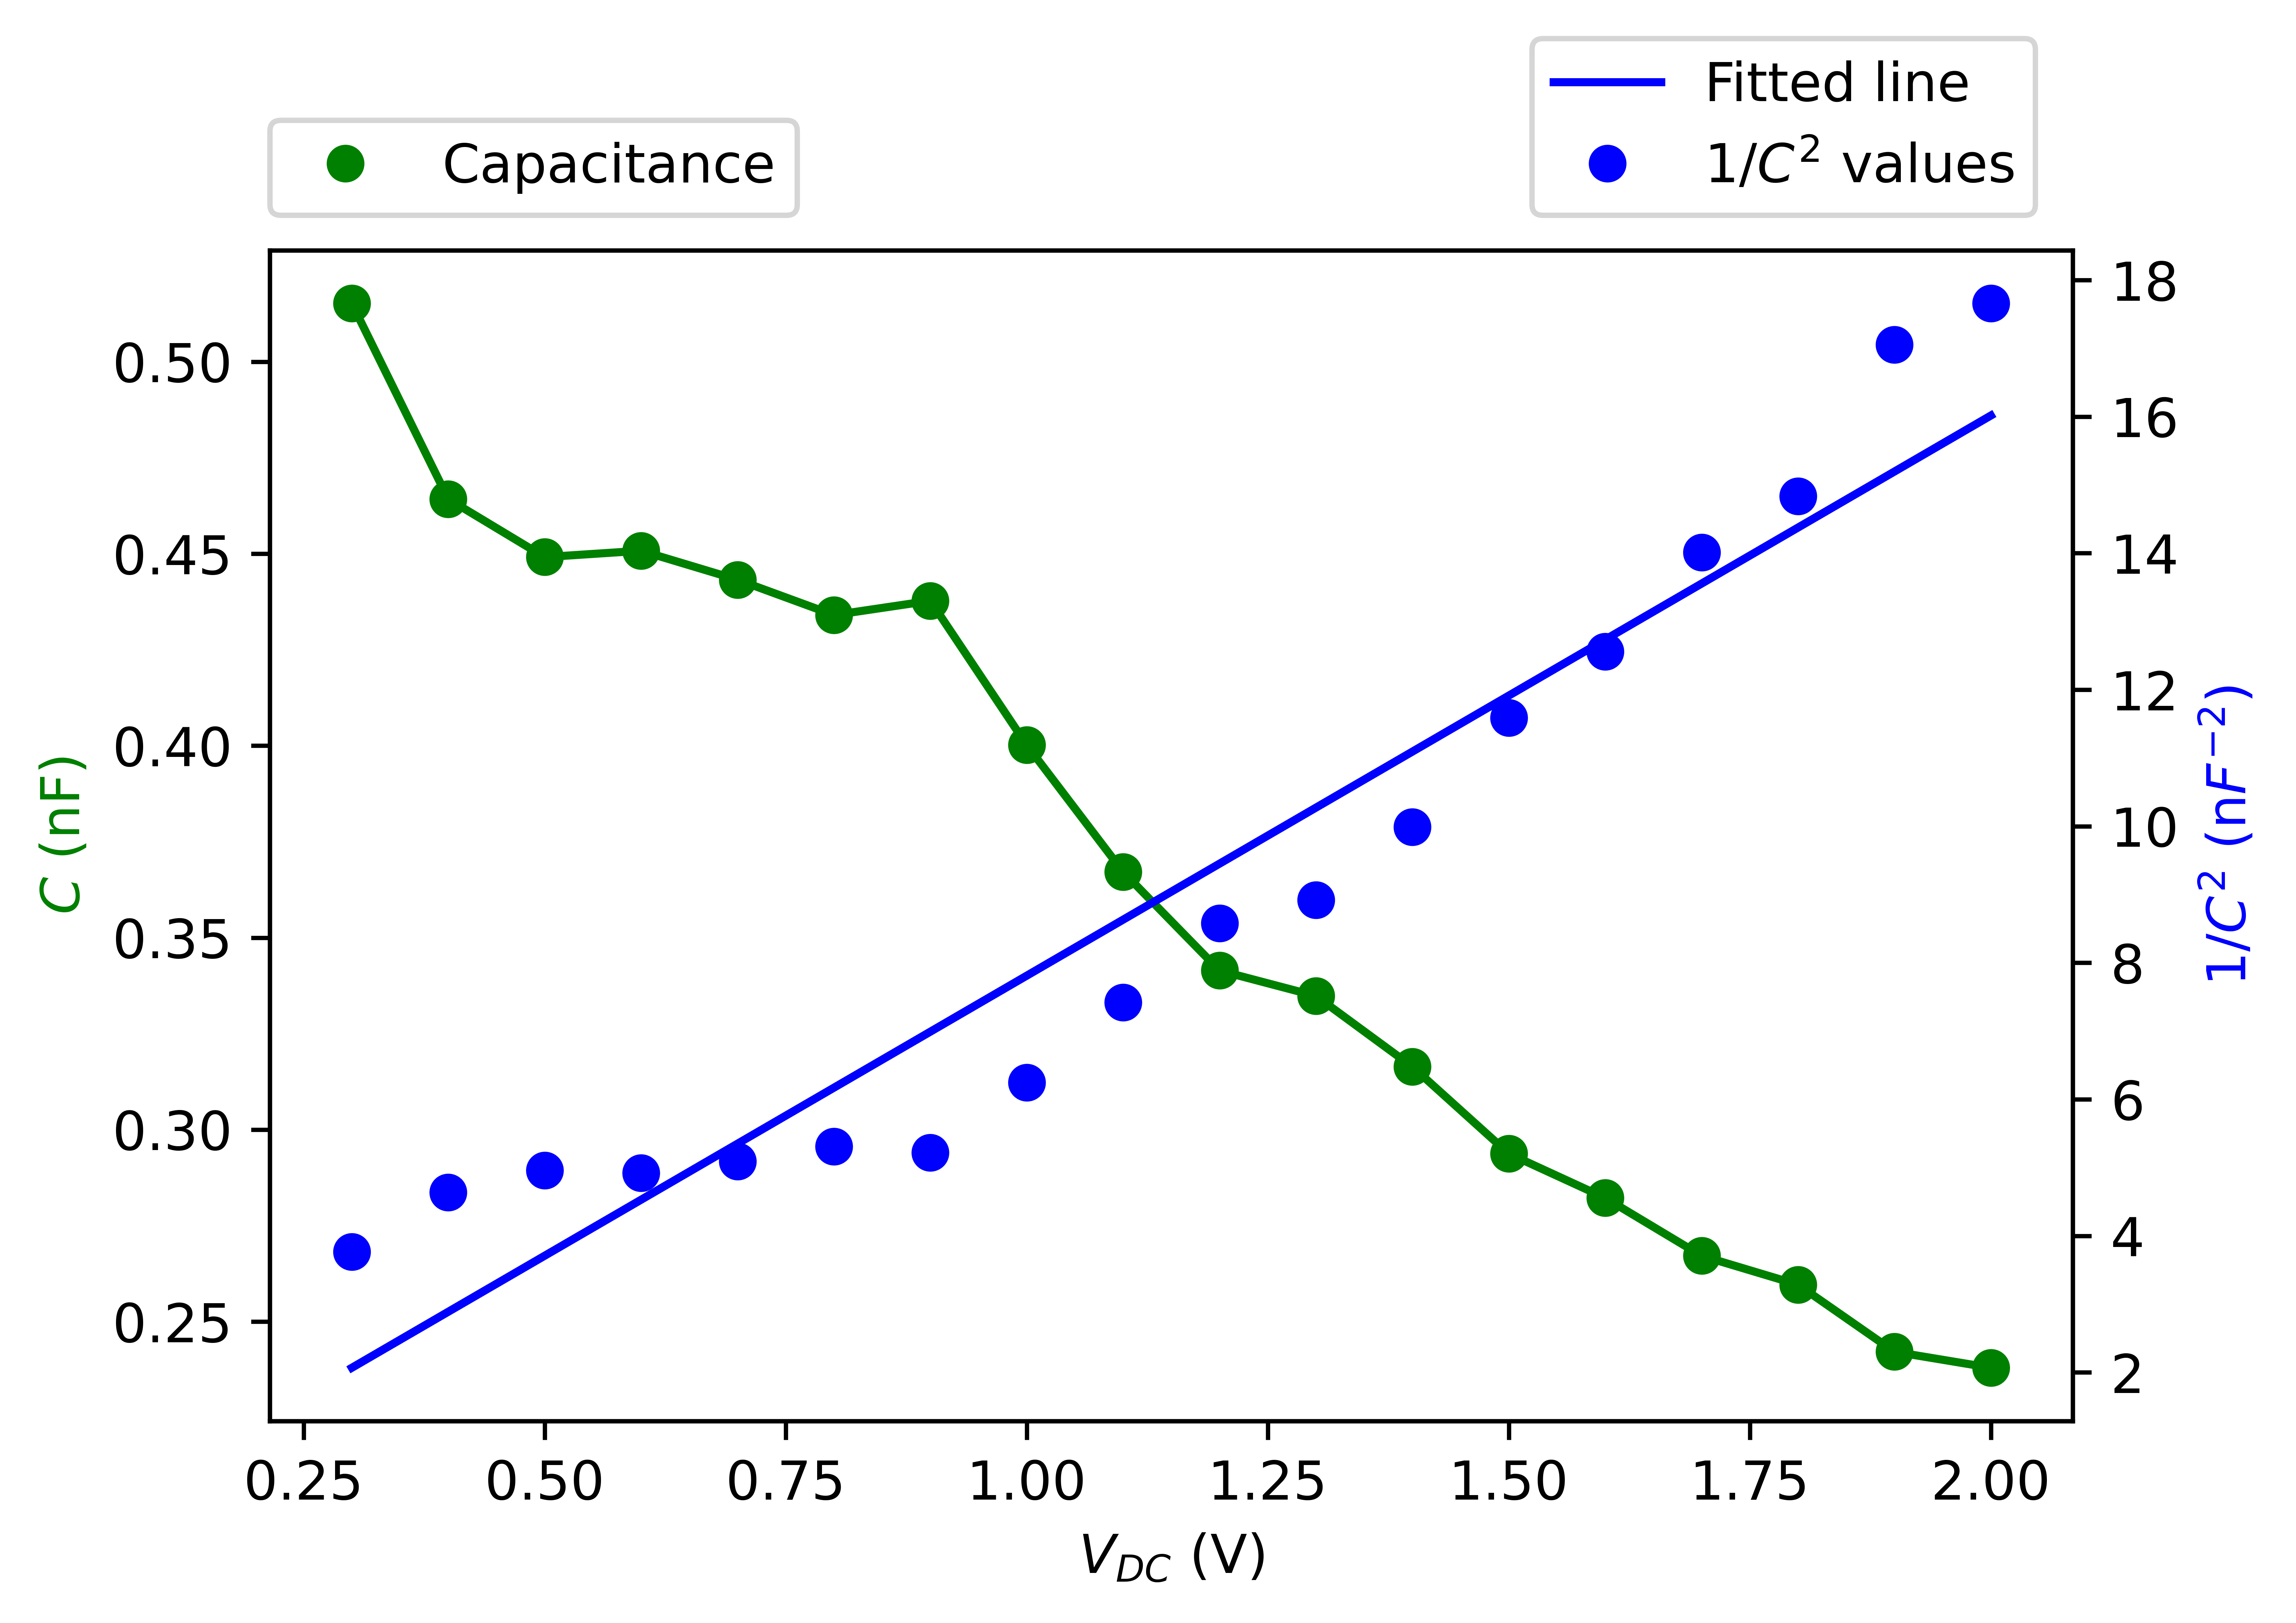
\includegraphics[scale = 0.54]{Figures/plot-cv-dark.png}
        \caption{C-V characteristic curve for the solar cell under dark conditions}
        \label{fig:cv-dark}
    \end{figure}
\section{Calculations}
    \begin{table*}[]
    \caption{Parameters of solar cell under illumination by the incandescent halogen lamp determined from the I-V characteristic curve}
    \label{tab:iv-1}
    \setlength{\tabcolsep}{12pt}
    \begin{tabular}{@{}ccccccccc@{}}
    \toprule
    \textbf{Filter} & \begin{tabular}[c]{@{}c@{}}$\mathbf{V_{OC}}$\\ ($\si{\volt}$)\end{tabular} & \begin{tabular}[c]{@{}c@{}}$\mathbf{I_{SC}}$\\ ($\si{\milli \ampere}$)\end{tabular} & \begin{tabular}[c]{@{}c@{}}\textbf{Power}, $P$\\ ($\si{\milli \watt}$)\end{tabular} & \begin{tabular}[c]{@{}c@{}}$\mathbf{V_{max}}$\\ ($\si{\volt}$)\end{tabular} & \begin{tabular}[c]{@{}c@{}}$\mathbf{I_{max}}$\\ ($\si{\milli \ampere}$)\end{tabular} & \begin{tabular}[c]{@{}c@{}}$\mathbf{P_{max}}$\\ ($\si{\milli \watt}$)\end{tabular} & \textbf{Fill factor}, $\mathbf{FF}$ & \textbf{Average fill factor} \\ \midrule
    \textit{No filter} & 3.759 & 0.268 & 1.007 & 2.944 & 0.203 & 0.598 & 59.323 \% & \multirow{5}{*}{60.247 \%} \\
    \textit{Red filter} & 3.73 & 0.268 & 1 & 3.123 & 0.196 & 0.612 & 61.233 \% &  \\
    \textit{Green filter} & 3.7 & 0.285 & 1.055 & 3.182 & 0.203 & 0.646 & 61.256 \% &  \\
    \textit{Yellow filter} & 3.77 & 0.263 & 0.992 & 3.248 & 0.192 & 0.624 & 62.896 \% &  \\
    \textit{Pink filter} & 3.93 & 0.356 & 1.399 & 3.176 & 0.249 & 0.791 & 56.525 \% &  \\ \bottomrule
    \end{tabular}
    \end{table*}
    \begin{table*}[]
    \caption{Parameters of solar cell under illumination by the sun determined from the I-V characteristic curve}
    \label{tab:iv-2}
    \setlength{\tabcolsep}{12pt}
    \begin{tabular}{@{}ccccccccc@{}}
    \toprule
    \textbf{Filter} & \begin{tabular}[c]{@{}c@{}}$\mathbf{V_{OC}}$\\ ($\si{\volt}$)\end{tabular} & \begin{tabular}[c]{@{}c@{}}$\mathbf{I_{SC}}$\\ ($\si{\milli \ampere}$)\end{tabular} & \begin{tabular}[c]{@{}c@{}}\textbf{Power}, $P$\\ ($\si{\milli \watt}$)\end{tabular} & \begin{tabular}[c]{@{}c@{}}$\mathbf{V_{max}}$\\ ($\si{\volt}$)\end{tabular} & \begin{tabular}[c]{@{}c@{}}$\mathbf{I_{max}}$\\ ($\si{\milli \ampere}$)\end{tabular} & \begin{tabular}[c]{@{}c@{}}$\mathbf{P_{max}}$\\ ($\si{\milli \watt}$)\end{tabular} & \textbf{Fill factor}, $\mathbf{FF}$ & \textbf{Average fill factor} \\ \midrule
    \textit{No filter} & 6 & 70.1 & 420.6 & 5.1 & 61.5 & 313.65 & 74.572 \% & \multirow{4}{*}{76.203 \%} \\
    \textit{Red filter} & 5.67 & 45.9 & 260.253 & 4.83 & 42.7 & 206.241 & 79.246 \% &  \\
    \textit{Yellow filter} & 5.73 & 51.1 & 292.803 & 4.78 & 46.5 & 222.27 & 75.911 \% &  \\
    \textit{Pink filter} & 5.78 & 52.9 & 305.762 & 4.98 & 46.1 & 229.578 & 75.084 \% &  \\ \bottomrule
    \end{tabular}
    \end{table*}
    \subsection{Efficiency of the solar cell under illumination by the Sun}
        Efficiency is defined as
        \begin{equation}
            \eta = \dfrac{\text{Power output}}{\text{Power input}}
        \end{equation}
        We can find the incident or power input using average solar irradiance which is $\SI{100}{\milli \watt \per \metre \squared}$. The area of the solar cell is $\SI{16}{\centi \metre \squared}$. Therefore, power input is $\SI{1600}{\milli \watt}$. The power output in absence of any filter when the solar cell was illuminated by the Sun was $\SI{313.65}{\milli \watt}$ as given in table (\ref{tab:iv-2}). From here
        \begin{equation}
            \boxed{\eta = \dfrac{313.65}{1600} = 19.6 \%}
        \end{equation}
    \subsection{Doping density and built-in voltage of the solar cell under light conditions}
        Using linear regression analysis, the equation of the straight line obtained by fitting the $1/C^2$ versus $V_{DC}$ data points in light conditions (figure (\ref{fig:cv-light})) is $y= 252.06475729323213x -108.26658750148931$. The unit of slope is $\si{\per \micro \farad \squared \per \volt}$. Therefore, $m = \SI{2.52e14}{\per \farad \squared \per \volt}$. Similarly, $Y$-intercept is $\SI{-1.08e-4}{\per \farad \squared}$.
        \par
        Now the doping density is given by
        \begin{equation}
            N_d = \dfrac{2}{q \epsilon_0 \epsilon_s A^2 m}
        \end{equation}
        where $m$ is the slope. Putting in the values, we get $N_d = \SI{1.25e19}{\per \metre \cubed}$.
        \par
        Similarly, the built-in voltage, $V_{bi}$, is given by
        \begin{equation}
            V_{bi} = \dfrac{c}{m}
        \end{equation}
        where $c$ is the $Y$-intercept and $m$ is the slope. Putting in the values, we get $V_{bi} = \SI{0.43}{\volt}$.
    \subsection{Doping density and built-in voltage of the solar cell under dark conditions}
        Using linear regression analysis, the equation of the straight line obtained by fitting the $1/C^2$ versus $V_{DC}$ data points in dark conditions (figure (\ref{fig:cv-dark})) is $y= 8.204535788895768x -0.3926397132301327$. The unit of slope is $\si{\per \micro \farad \squared \per \volt}$. Therefore, $m = \SI{8.20e18}{\per \farad \squared \per \volt}$. Similarly, $Y$-intercept is $\SI{-3.93e-10}{\per \farad \squared}$.
        \par
        Now the doping density is given by
        \begin{equation}
            N_d = \dfrac{2}{q \epsilon_0 \epsilon_s A^2 m}
        \end{equation}
        where $m$ is the slope. Putting in the values, we get $N_d = \SI{3.86e14}{\per \metre \cubed}$.
        \par
        Similarly, the built-in voltage, $V_{bi}$, is given by
        \begin{equation}
            V_{bi} = \dfrac{c}{m}
        \end{equation}
        where $c$ is the $Y$-intercept and $m$ is the slope. Putting in the values, we get $V_{bi} = \SI{0.048}{\volt}$.
    
\section{Error Analysis}
    \subsection{In Doping density and built-in voltage of the solar cell under light conditions}
        Error in doping density $N_d$ is given by
        \begin{equation}
            \delta N_d = \dfrac{\delta m}{m} \times N_d \\
        \end{equation}
        Using NumPy library's regression analysis, the error in slope was obtained as $\delta m = \SI{1.26e13}{\per \farad \squared \per \volt}$. Putting in the values we get $\delta N_d = \SI{0.05e19}{\per \metre \cubed}$.
        \par
        Similarly, error in built-in voltage, $V_{bi}$, is given by
        \begin{equation}
            \delta V_{bi} = V_{bi} \sqrt{\Big( \dfrac{\delta y}{y} \Big)^2 + \Big( \dfrac{\delta m}{m} \Big)^2}
        \end{equation}
        Here, $\delta y$ is the error in $Y$-intercept and using NumPy library's regression analysis it was found to be $\delta y = \SI{-1.59e-5}{\per \farad \squared}$. Putting in the values, we get $\delta V_{bi} = \SI{0.07}{\volt}$. 
    \subsection{In Doping density and built-in voltage of the solar cell under dark conditions}
        Error in doping density $N_d$ is given by
        \begin{equation}
            \delta N_d = \dfrac{\delta m}{m} \times N_d \\
        \end{equation}
        Using NumPy library's regression analysis, the error in slope was obtained as $\delta m = \SI{0.58e18}{\per \farad \squared \per \volt}$. Putting in the values we get $\delta N_d = \SI{2.72e13}{\per \metre \cubed}$.
        \par
        Similarly, error in built-in voltage, $V_{bi}$, is given by
        \begin{equation}
            \delta V_{bi} = V_{bi} \sqrt{\Big( \dfrac{\delta y}{y} \Big)^2 + \Big( \dfrac{\delta m}{m} \Big)^2}
        \end{equation}
        Here, $\delta y$ is the error in $Y$-intercept and using NumPy library's regression analysis it was found to be $\delta y = \SI{0.73e-9}{\per \farad \squared}$. Putting in the values, we get $\delta V_{bi} = \SI{0.009}{\volt}$. 
    
\section{Results}
    \begin{enumerate}
        \item The average fill factor for the solar cell under Incandescent lamp was found to be 60.247 \%.
        \item The average fill factor for the solar cell under sun was found to be 76.203 \%.
        \item The power obtained under sun was much greater than lamp, as the intensity of sun is much higher.
        \item The efficiency of the solar cell under illumination by the Sun was found to be $\eta = 19.6 \%$.
        \item The doping density in the solar cell under light conditions was found to be $N_d = \SI[separate-uncertainty=true]{1.25 \pm 0.05e19}{\per \metre \cubed}$.
        \item The doping density in the solar cell under dark conditions was found to be $N_d = \SI[separate-uncertainty=true]{3.86 \pm 0.27e14}{\per \metre \cubed}$.
        \item The built-in voltage of the solar cell in light conditions was found to be $V_{bi} = \SI[separate-uncertainty=true]{0.43 \pm 0.07}{\volt}$.
        \item The built-in voltage of the solar cell in light conditions was found to be $V_{bi} = \SI[separate-uncertainty=true]{0.048 \pm 0.009}{\volt}$.
    \end{enumerate}

\section{Discussions}
    \begin{enumerate}
        \item In the region (of I-V characteristics graph) where the I starts falling drastically, we can employ a potentiometer of larger resistance that can be better tuned to get more number of points in that region.
        \item Under sun the current falls drastically, and readings must be taken carefully to obtain the maximum power.
        \item $I_{SC}$ was not constant with change in wavelength of light, even though it is dependent on intensity and not wavelength. This can be explained as there is a dependence of intensity on wavelength.
        \item The photo diode in dark conditions works as normal p-n junction diode with applied reverse bias voltage.
        \item The $V_{OUT}$ of the solar cell in light condition was observed to be constant indicating that the maximum output voltage was achieved.
        \item The transimpedance amplifier part of the circuit acts as an active low pass filter. The gain, $V_{OUT}/V_{DUT}$ is high for low $\omega$.
        \item The decreasing trend of the $C$ versus $V_{DC}$ plots can be explained by the fact that as the applied voltage is reverse biased, the width of the depletion region increases with increase in the input $V_{DC}$ which results in decreased capacitance.
    \end{enumerate}

    
\section{Precautions}
    \begin{enumerate}
        \item Quite a few points are missed when there is a sudden variation in the current output because of small value of potentiometer used; this causes an error in determining the nature of graph.
        \item The experiment done under the sun is subject to the weather conditions and causes error in readings as the weather fluctuates during the course of experiment.
        \item Filter paper are another cause of error as the incident light on solar cell does not remain uniform instead plastic/glass filters should be used.
        \item Do not disturb the setup while taking the measurements.
        \item For dark conditions use a thick black cloth only.
        \item Do not operate the diode in breakdown region.
        \item This is a test.
    \end{enumerate}

\end{document}
%
% ****** End of file aipsamp.tex ******